\section{作业及答案：结构力学基础与技巧班第8次作业及答案（静定结构影响线）}
\begin{analysisbox}
影响线可用静力法或机动法。剪力影响线关注截面两侧相对竖向位移，弯矩影响线关注相对转角；移动荷载取影响线同号面积最大的位置。
\end{analysisbox}
\subsection*{第 1 页转写}
第三章

静定结构的影响线

扣

＋

N

=

F

-

，

沪max=

lOXO. 5 =25kN。

五、练习题

图3-48所示结构在任意长度可移动荷载20kN/m作用下，截面K的剪力最大

值FQKmax 为

。（天津大学2010)

3-2求图3-48 所示结构在任意长度可动均布荷载20kN/m作用下截面K的最大弯

矩MKmax l。（华南理工大学2013)

3-3

图3-49所示多跨梁，截面K的剪力影响线在K点的竖标为YK左

＝

，

y店; =

; 在图示移动荷载作用下，截面K的剪力最大值为

。（浙江大学2009)

3-1

123
\begin{figure}[H]\centering
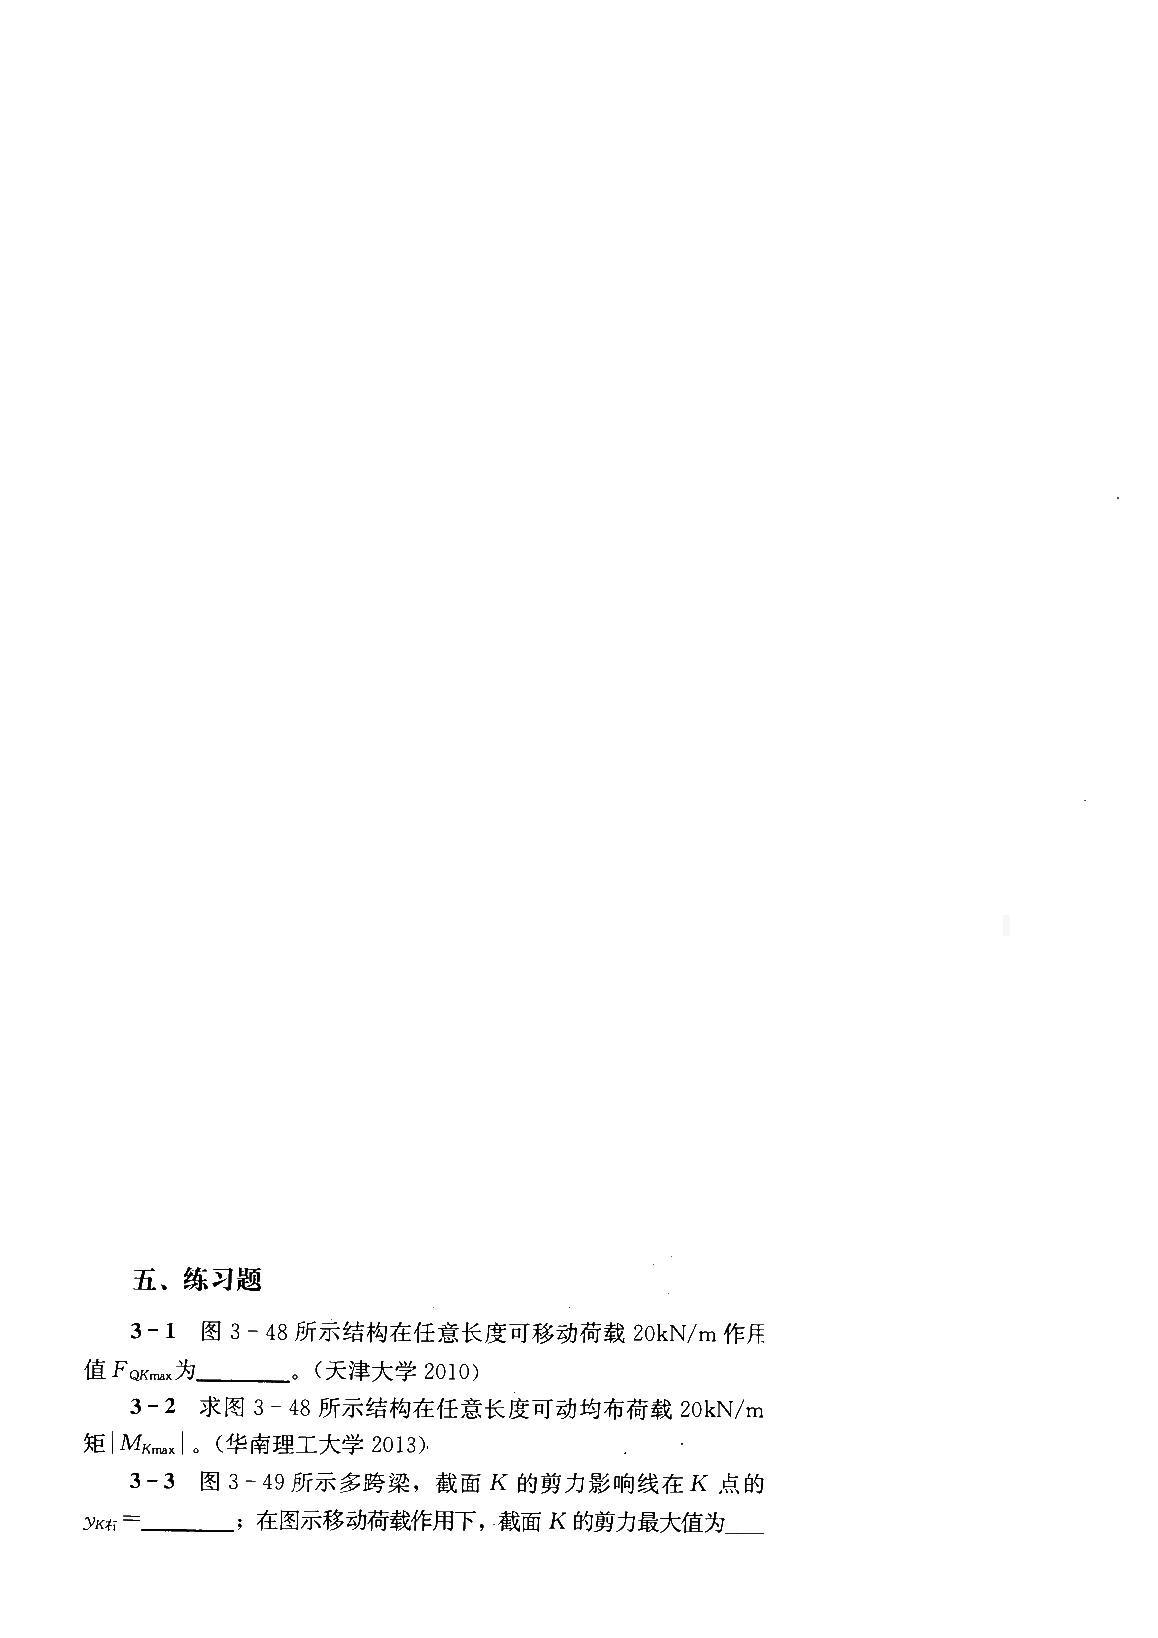
\includegraphics[width=0.92\textwidth]{figures/src11_p001.jpg}
\caption{结构力学基础与技巧班第8次作业及答案（静定结构影响线） 第 1 页清理图形页}
\end{figure}
\subsection*{第 2 页转写}
研究生入学考试辅导丛书结构力学（第二版）

Fpl-50kN/

Fp2=20kN

20kN/m

8m

6m

8m

2ml2ml

8m

图3-48

图3-49

3-4

用机动法作图3-50所示多跨静定梁中MA、F\&B、ME、MH的影响线。（湖南大

学2008)

3-5

作图3-51所示结构的FQk左、FQk右、Mk（下侧受拉为正）影响线。（广州大学

2011)

[Fp=1

Fp-=1

2m

2m

3m

2m

Llm/1m/1m/lm

2m

1m

2m

图3-50

图3-51

3-6用静力法作图3-52所示结构的MG、FQE、MA影响线。Mc以杆DC下侧受拉为

正；MA以AK杆端下侧受拉为正。（Fp=1在FDCH段上移动）（青岛理工大学2012）

3-7

作图3-53所示结构的Me、Mp影响线。（华南理工大学2008）

[ Fp=1

[Fp=]

3.5m

2m

图3-52

图3-53

3-8移动荷载Fp=1在下弦移动，试作图3-54所示桁架杆件内力FNa和FNe的影响

线。（河北工业大学2008）

2.4m

2mx6=12m

图3-54

3-9

作图3-55所示结构FRA、Fn1、Fn2、FN3的影响线。（单位力在上下弦

南大学2009)

3-10

作图3-56所示结构FA、FRB、McB的影响线。（广州大学2012）

124
\begin{figure}[H]\centering
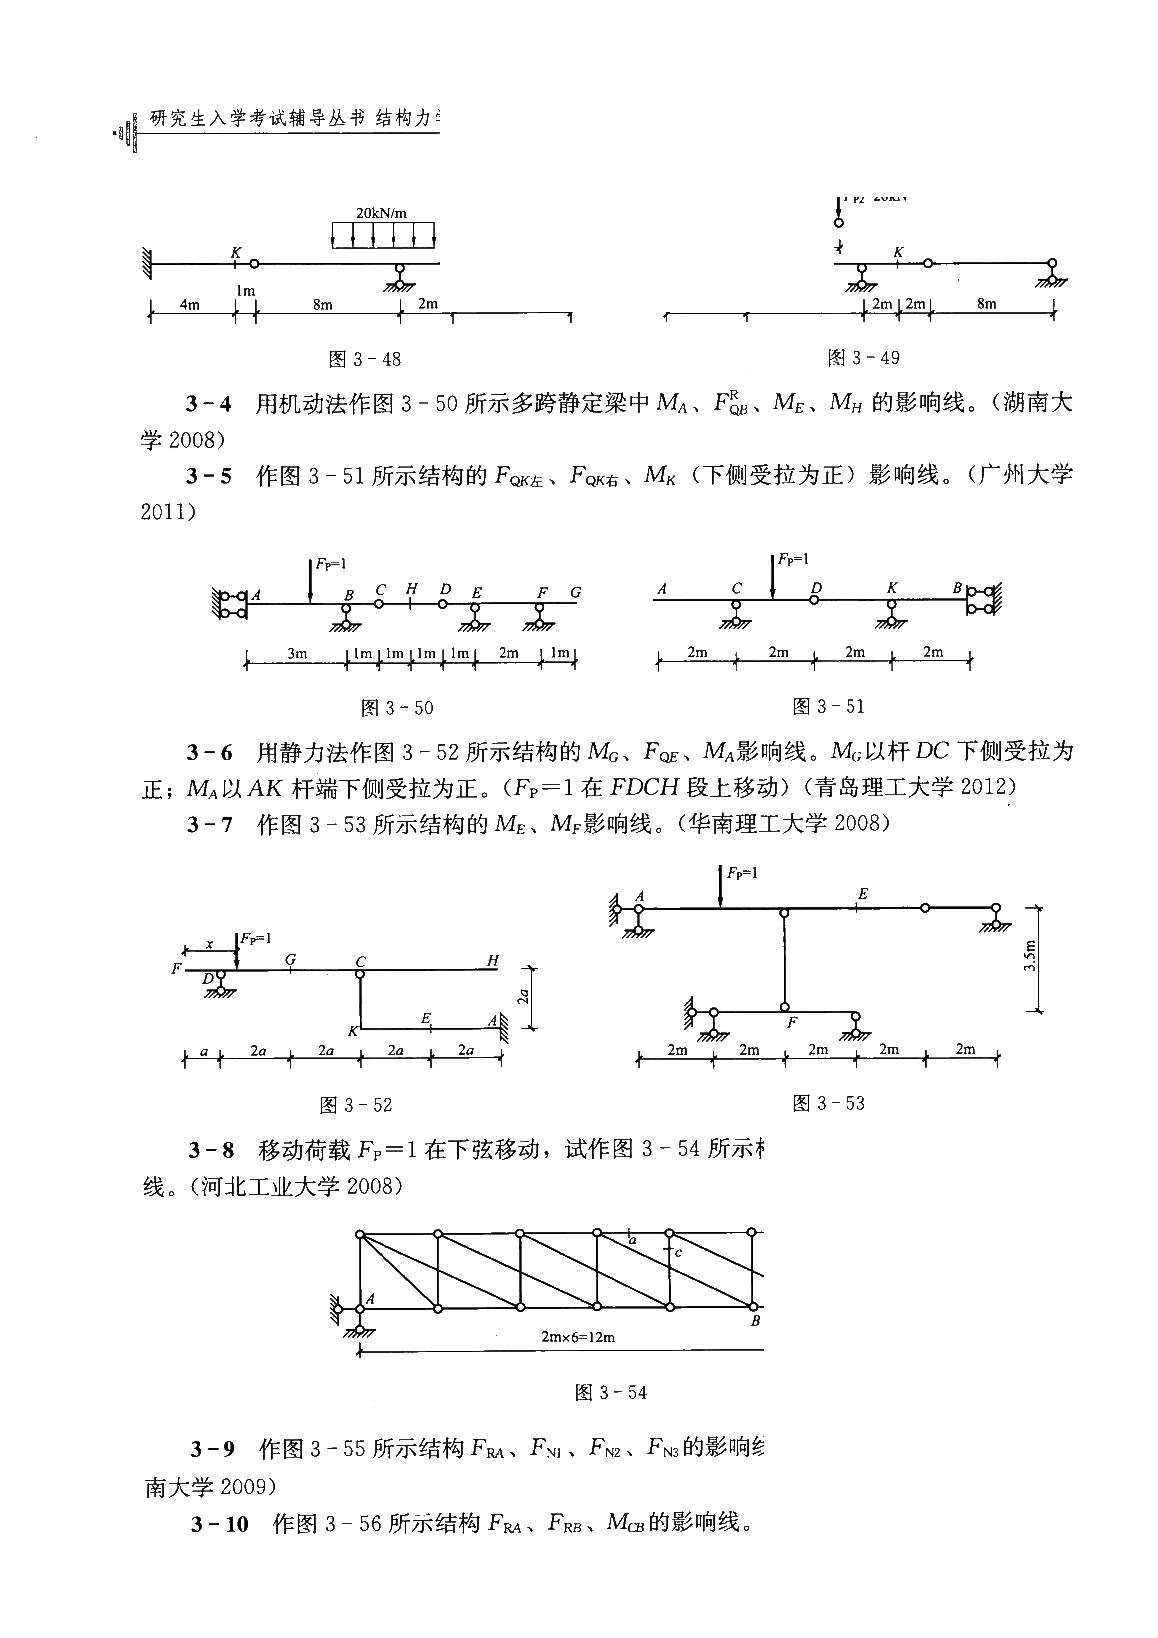
\includegraphics[width=0.92\textwidth]{figures/src11_p002.jpg}
\caption{结构力学基础与技巧班第8次作业及答案（静定结构影响线） 第 2 页清理图形页}
\end{figure}
\subsection*{第 3 页转写}
永久微销1电结柜网388

[Fp=]

6xa

图3-55

3-11图3-57所示结构，单位荷载Fp=1方向向下，沿B、C、D运动。（1）作轴

力FNDE、剪力FQBc和MBc的影响线。（2）若CD杆受到图示荷载作用，利用影响线计算

FNDE和MBC。（武汉理工大学2011）

[Fp=1

4kN/m

4m

OB

4m

3m

4m

4m

4m

3m

图3-56

图3-57

3-12试求3-58所示结构内力影响线MB、FNBA、FQBC（单位荷载Fp=1在DF段移

动）。（青岛理工大学2008）

3-13

图3-59所示结构，Fp=1沿BCD移动，试作出截面K弯矩（下侧受拉为正）

和轴力的影响线。（浙江大学2012）

[Fp=1

1/2

1/2

图3-58

图3-59

3-14用静力法作图3-60所示组合结构的MB、FN1、Fn2的影响线。（青岛理工大学

2009)

3-15图3-61所示为一个三铰拱：（1）设方向向下单位集中力Fp=1可以在拱上沿$\alpha$

轴方向移动，求作支座A水平反力FHA的影响线（$\alpha$轴以A为原点，以向右为正向）。（2）

设拱上布满方向向下、沿轴方向均匀分布的荷载q，试利用（1）中所求影响线，求解水

平反力FHA的值。（武汉理工大学2008）

3 - 16

（1）作图3-62所示结构支座D反力FR和K点弯矩Mk的影响线；（2）速

示移动荷载组作用下Mk的最大值。（要考虑荷载掉头）（西南交通大学2012)
\begin{figure}[H]\centering
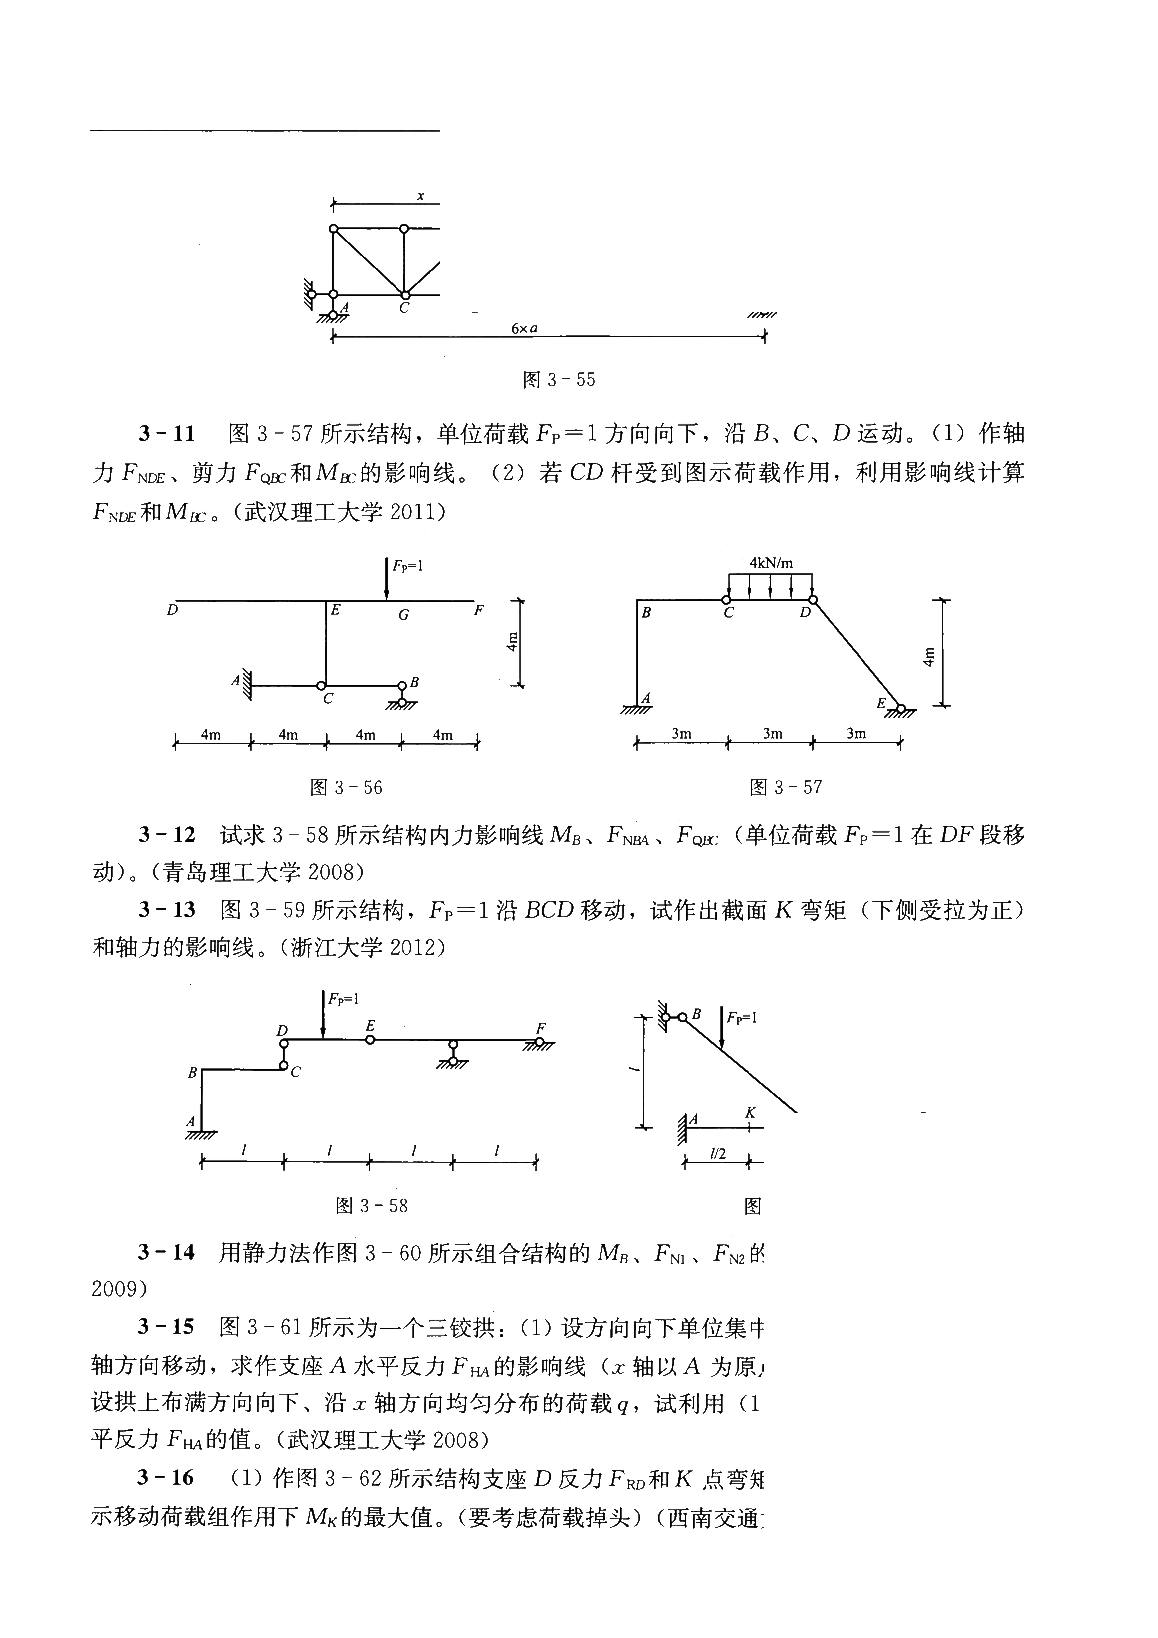
\includegraphics[width=0.92\textwidth]{figures/src11_p003.jpg}
\caption{结构力学基础与技巧班第8次作业及答案（静定结构影响线） 第 3 页清理图形页}
\end{figure}
\subsection*{第 4 页转写}
研究生入学考试辅导丛书结构力学（第二版）

Fp=1

Fp=1

FHB

1/2

3m

3m

1/2

图3-60

图3-61

30kN

10kN

J30kN

1m

2m

6m

4m

4m

4m

4m

4m

图3-62

126
\begin{figure}[H]\centering
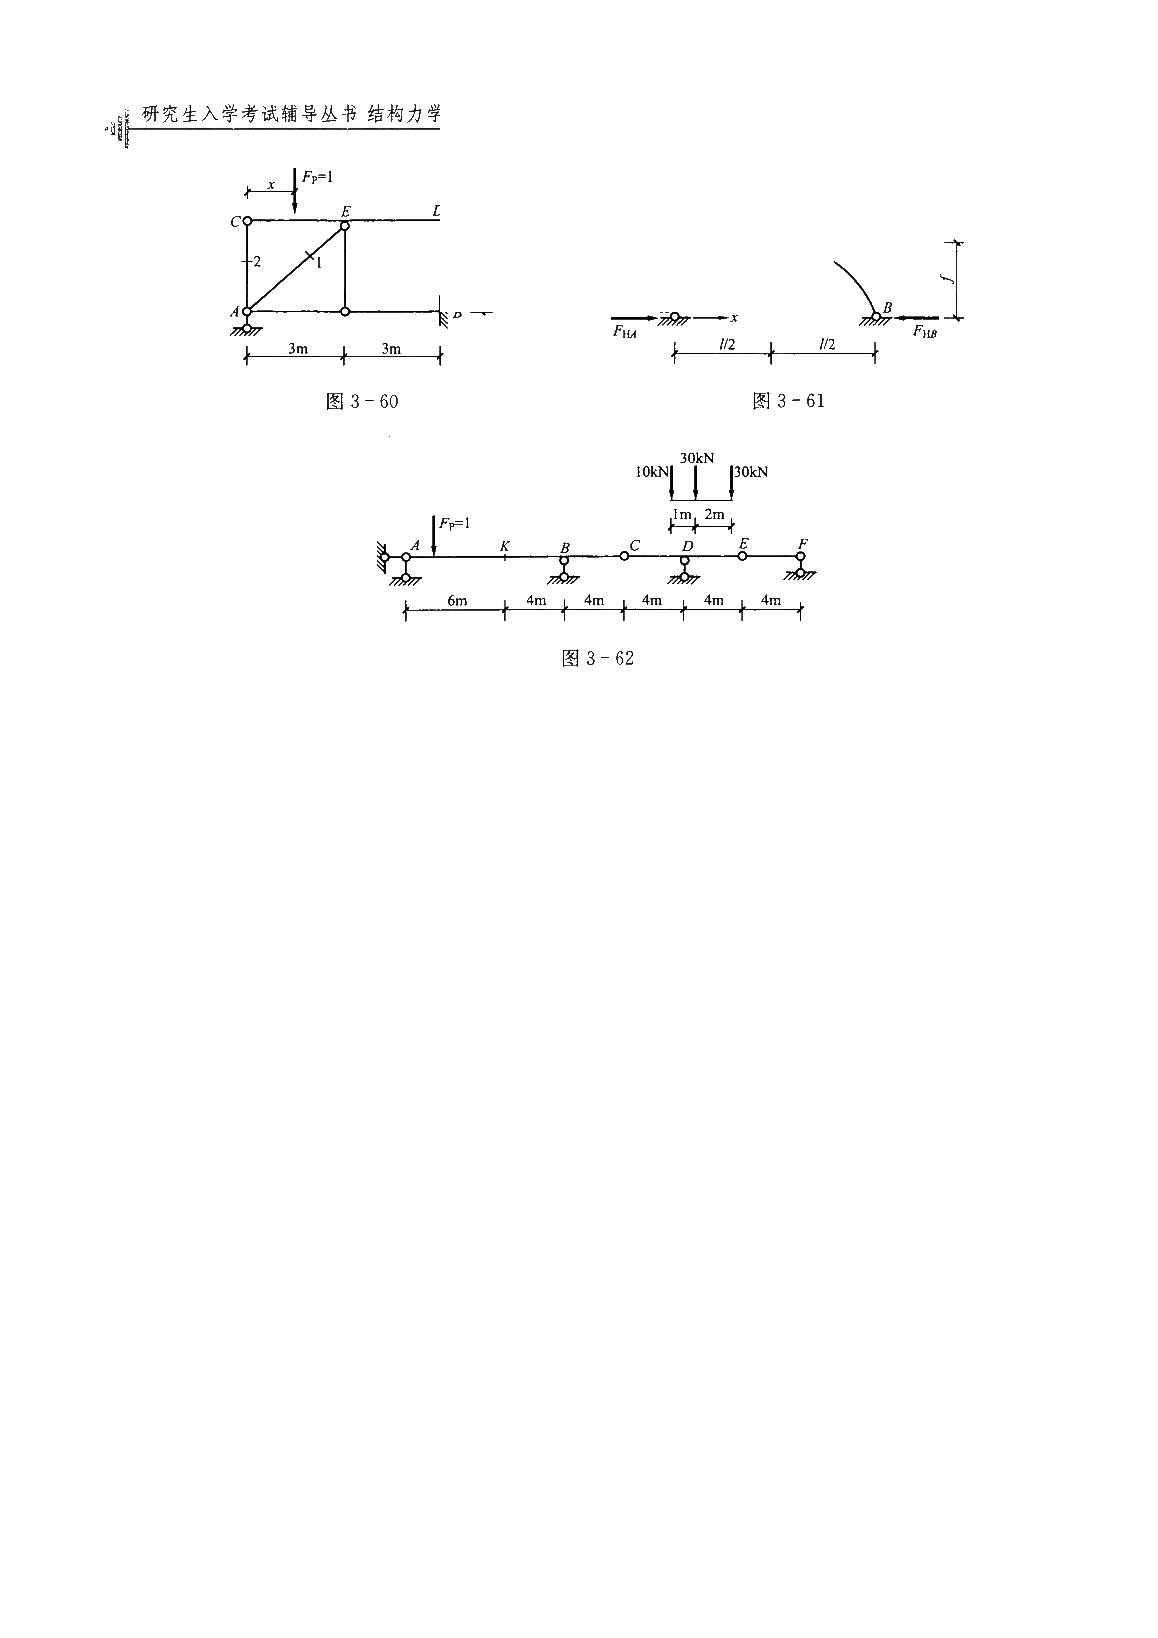
\includegraphics[width=0.92\textwidth]{figures/src11_p004.jpg}
\caption{结构力学基础与技巧班第8次作业及答案（静定结构影响线） 第 4 页清理图形页}
\end{figure}
\subsection*{第 5 页转写}
五、练习题

31、

2m

l =$\times$I*(b+1)$\times$ =0

3-2

ym

2m

33

个个

Q=5$\times$1+=70

3-
\begin{figure}[H]\centering
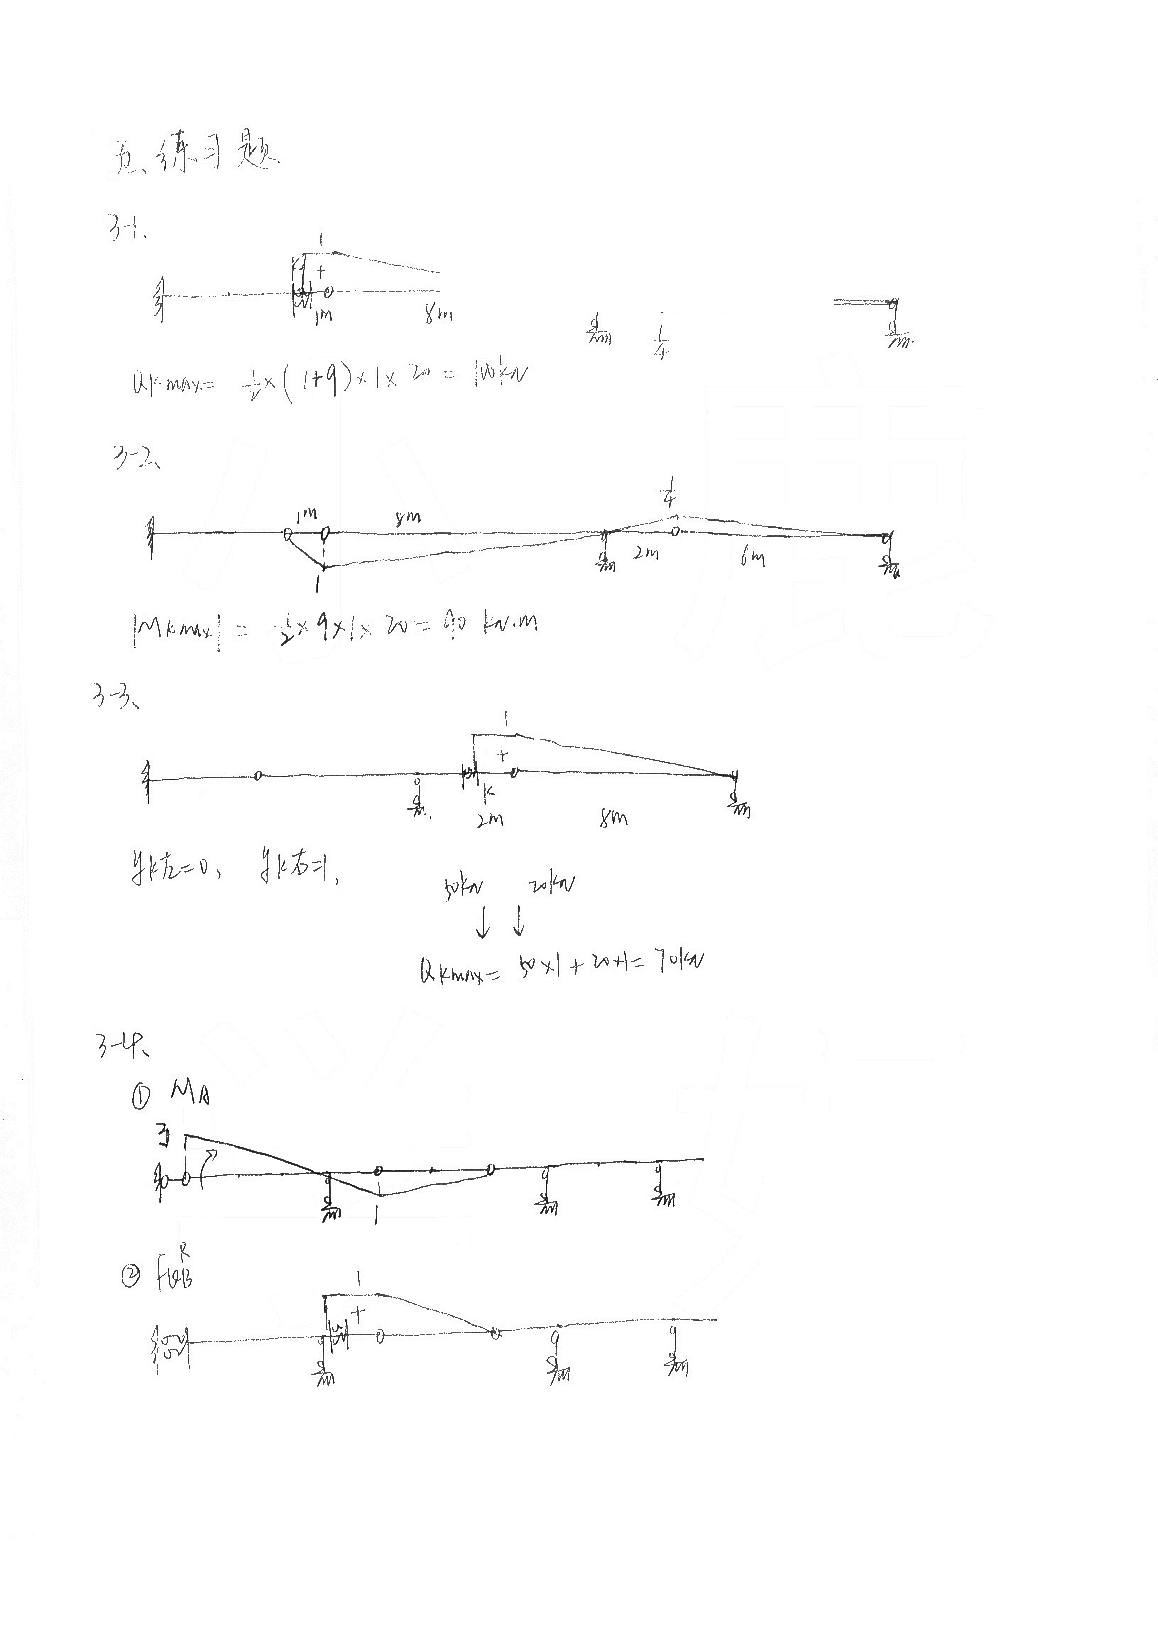
\includegraphics[width=0.92\textwidth]{figures/src11_p005.jpg}
\caption{结构力学基础与技巧班第8次作业及答案（静定结构影响线） 第 5 页清理图形页}
\end{figure}
\subsection*{第 6 页转写}
3-b、

DLX C30

Mc0-Foy$\times$ 44e

40

280

Fo图(EN)

FN图(KN)
\begin{figure}[H]\centering
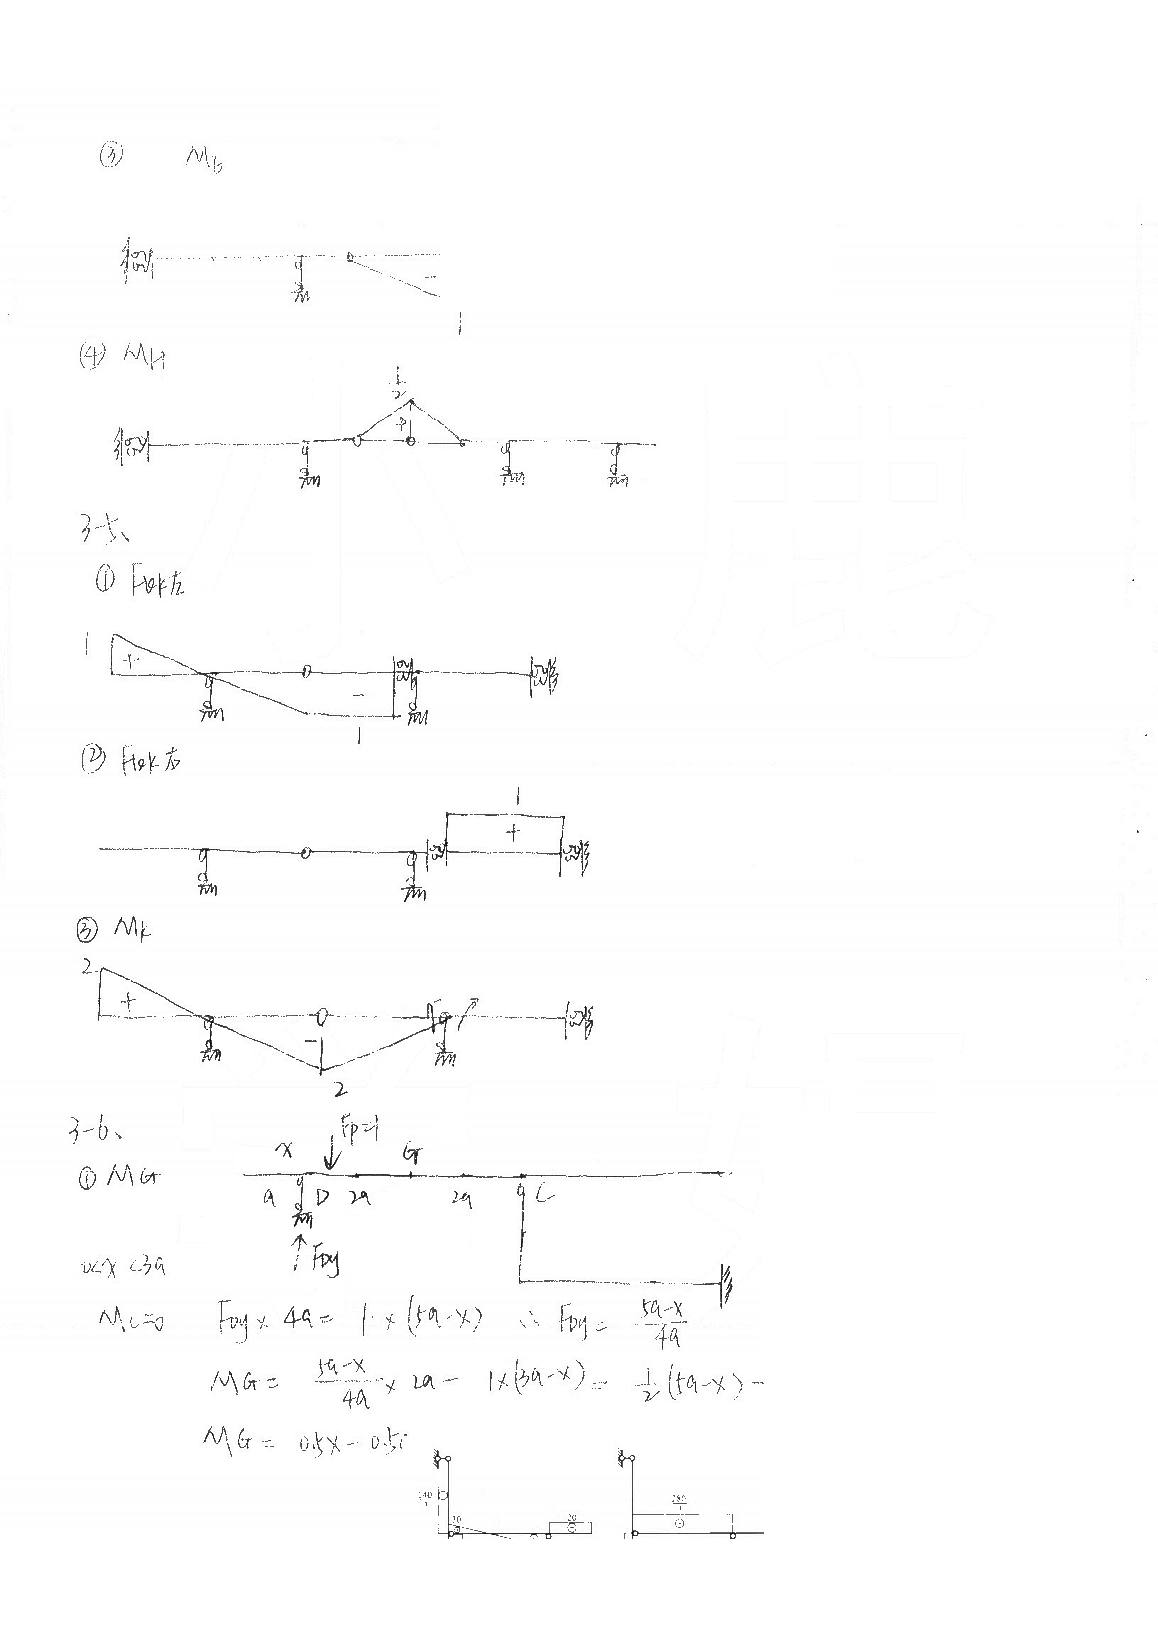
\includegraphics[width=0.92\textwidth]{figures/src11_p006.jpg}
\caption{结构力学基础与技巧班第8次作业及答案（静定结构影响线） 第 6 页清理图形页}
\end{figure}
\subsection*{第 7 页转写}
40

5a-x

Mu=0 ,Fry$\times$ 49+ 1x[x-t4)0, =

g, MG=

24

FRES

40

n-x

Hote

792X

50-X

-X

$\times$84 - 1(99-$\times$)=4-x

ME=

44

84
\begin{figure}[H]\centering
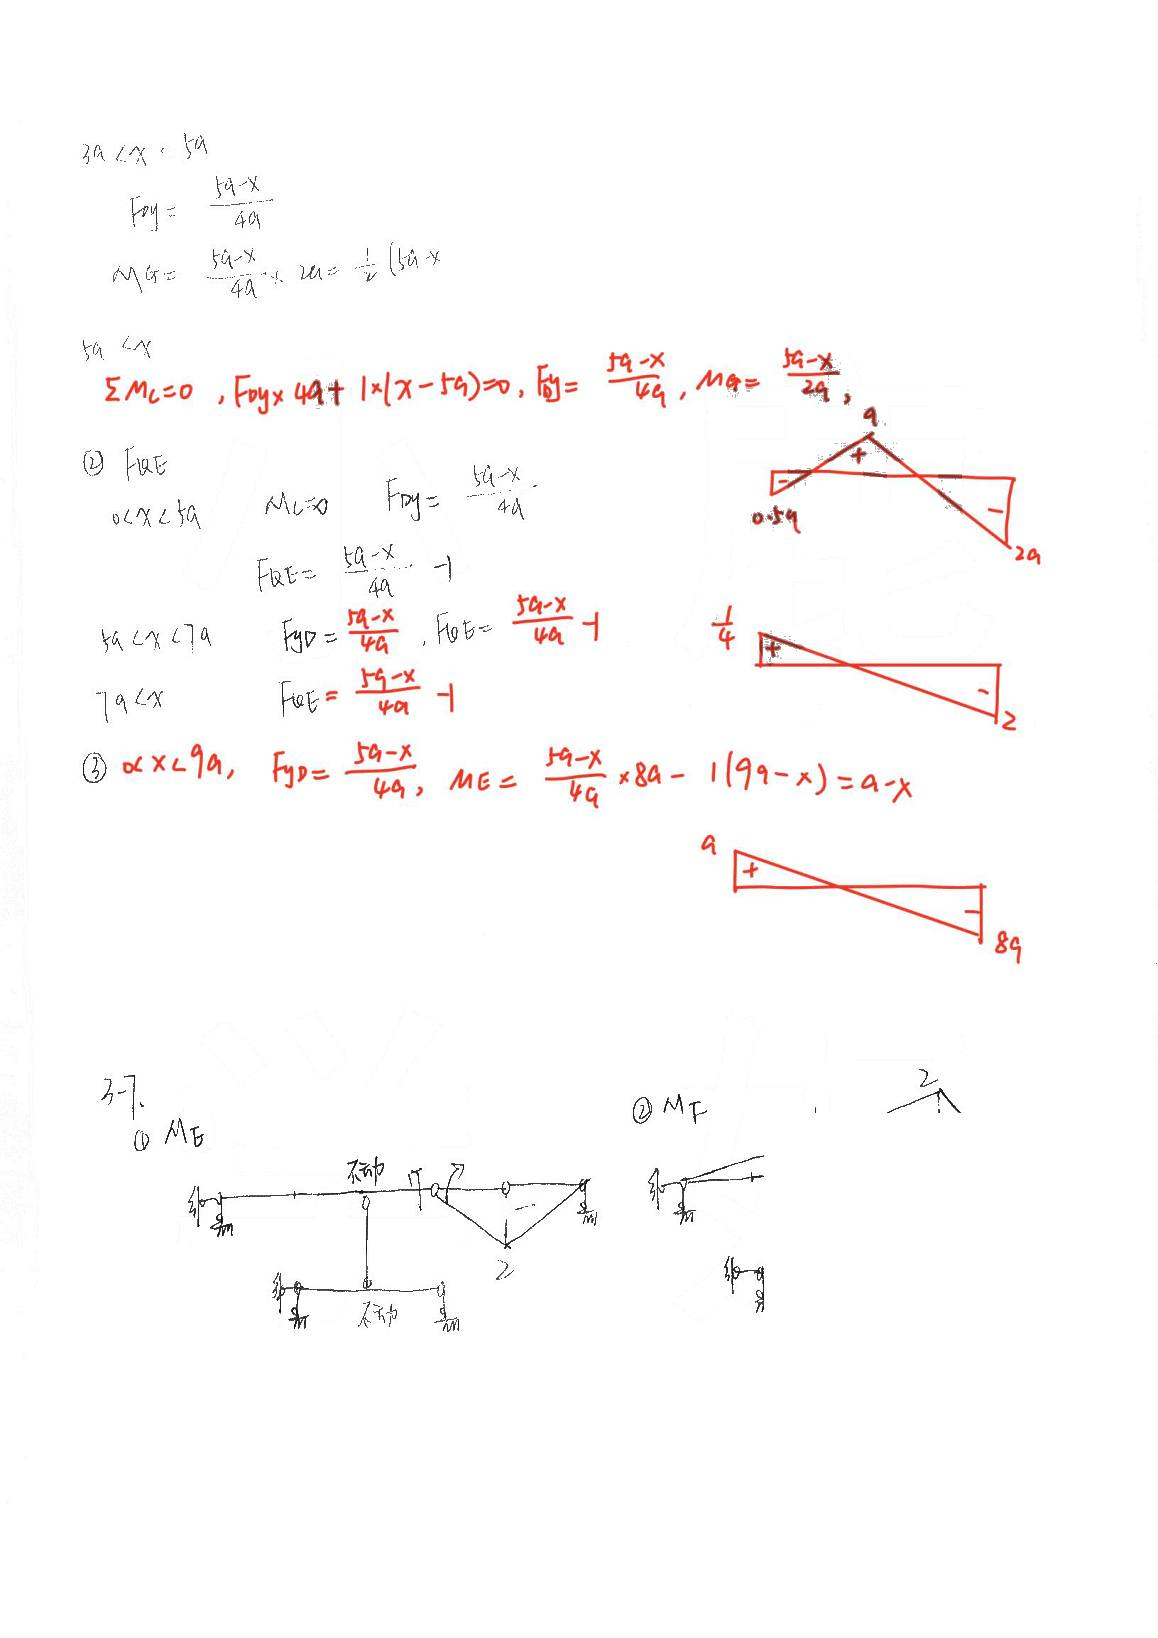
\includegraphics[width=0.92\textwidth]{figures/src11_p007.jpg}
\caption{结构力学基础与技巧班第8次作业及答案（静定结构影响线） 第 7 页清理图形页}
\end{figure}
\subsection*{第 8 页转写}
当单位力作用在上弦。

O PA

科在点左例时，开要

斗在右例时,取也

Fvit Fa,Fvi=
\begin{figure}[H]\centering
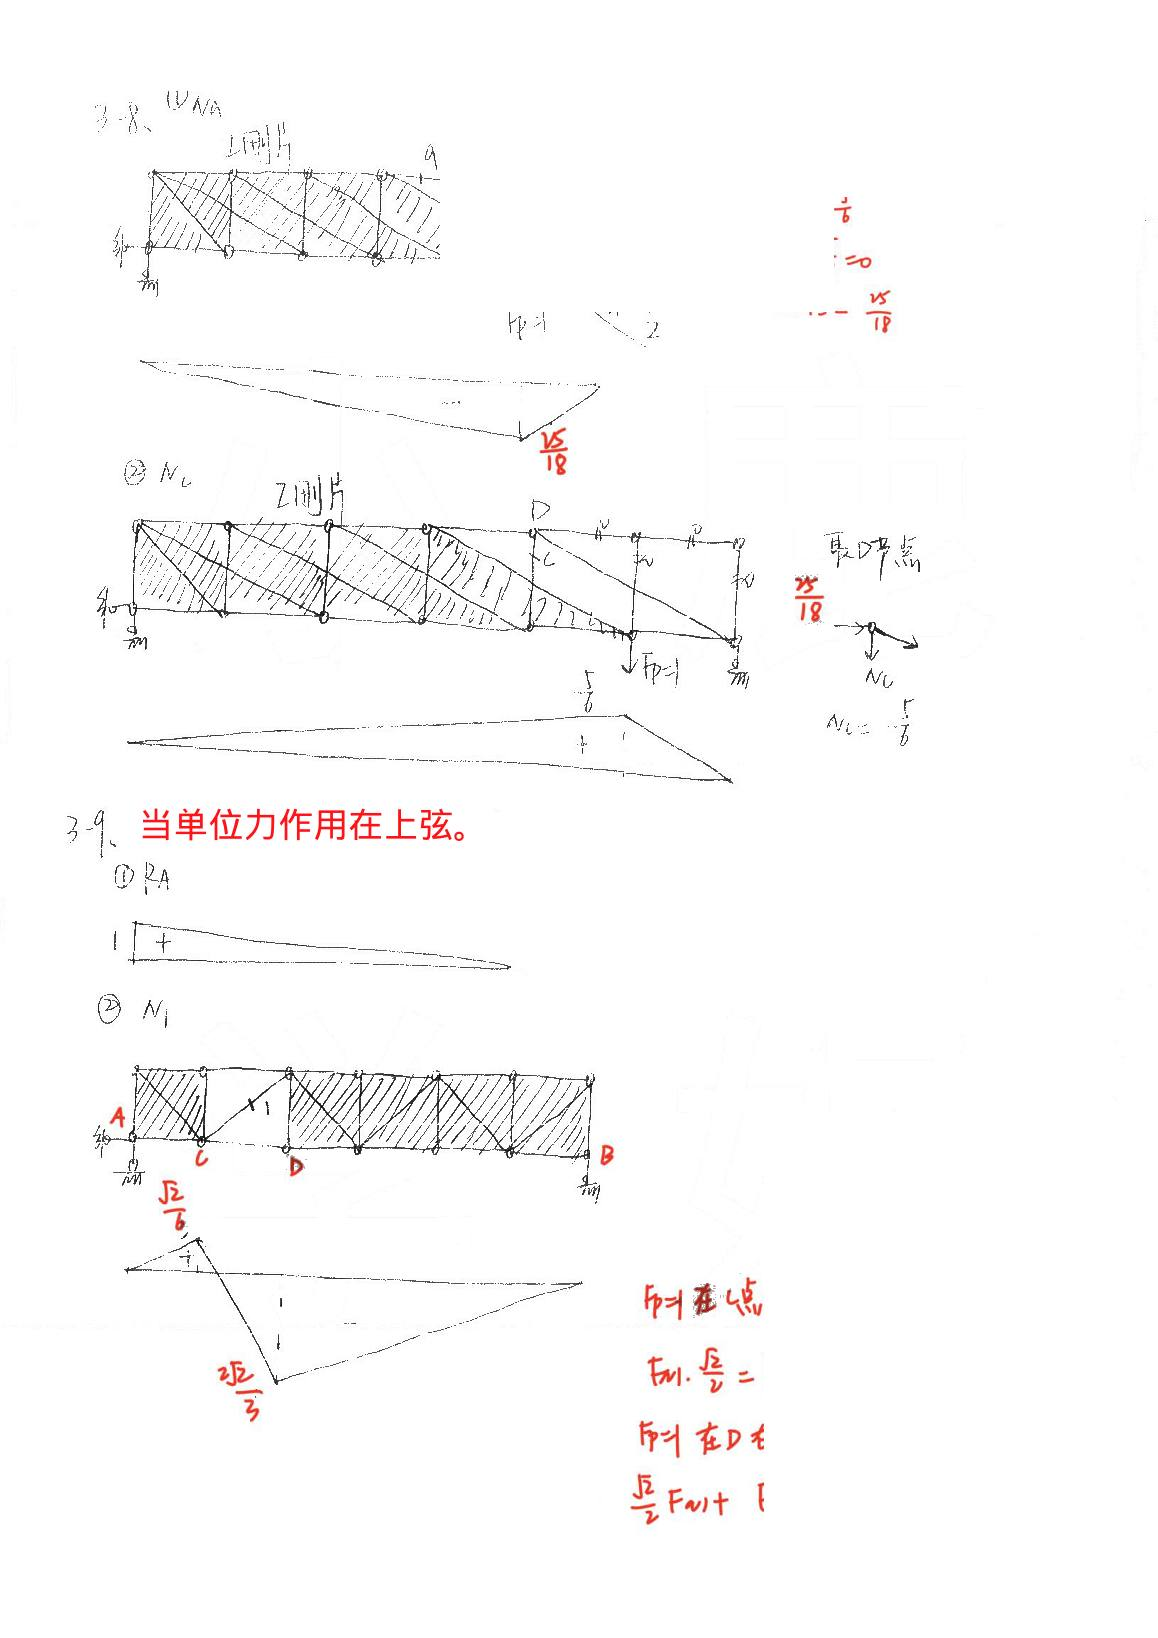
\includegraphics[width=0.92\textwidth]{figures/src11_p008.jpg}
\caption{结构力学基础与技巧班第8次作业及答案（静定结构影响线） 第 8 页清理图形页}
\end{figure}
\subsection*{第 9 页转写}
在6左例,取右史,

Fm=F，在右创时，

例，F= Fs
\begin{figure}[H]\centering
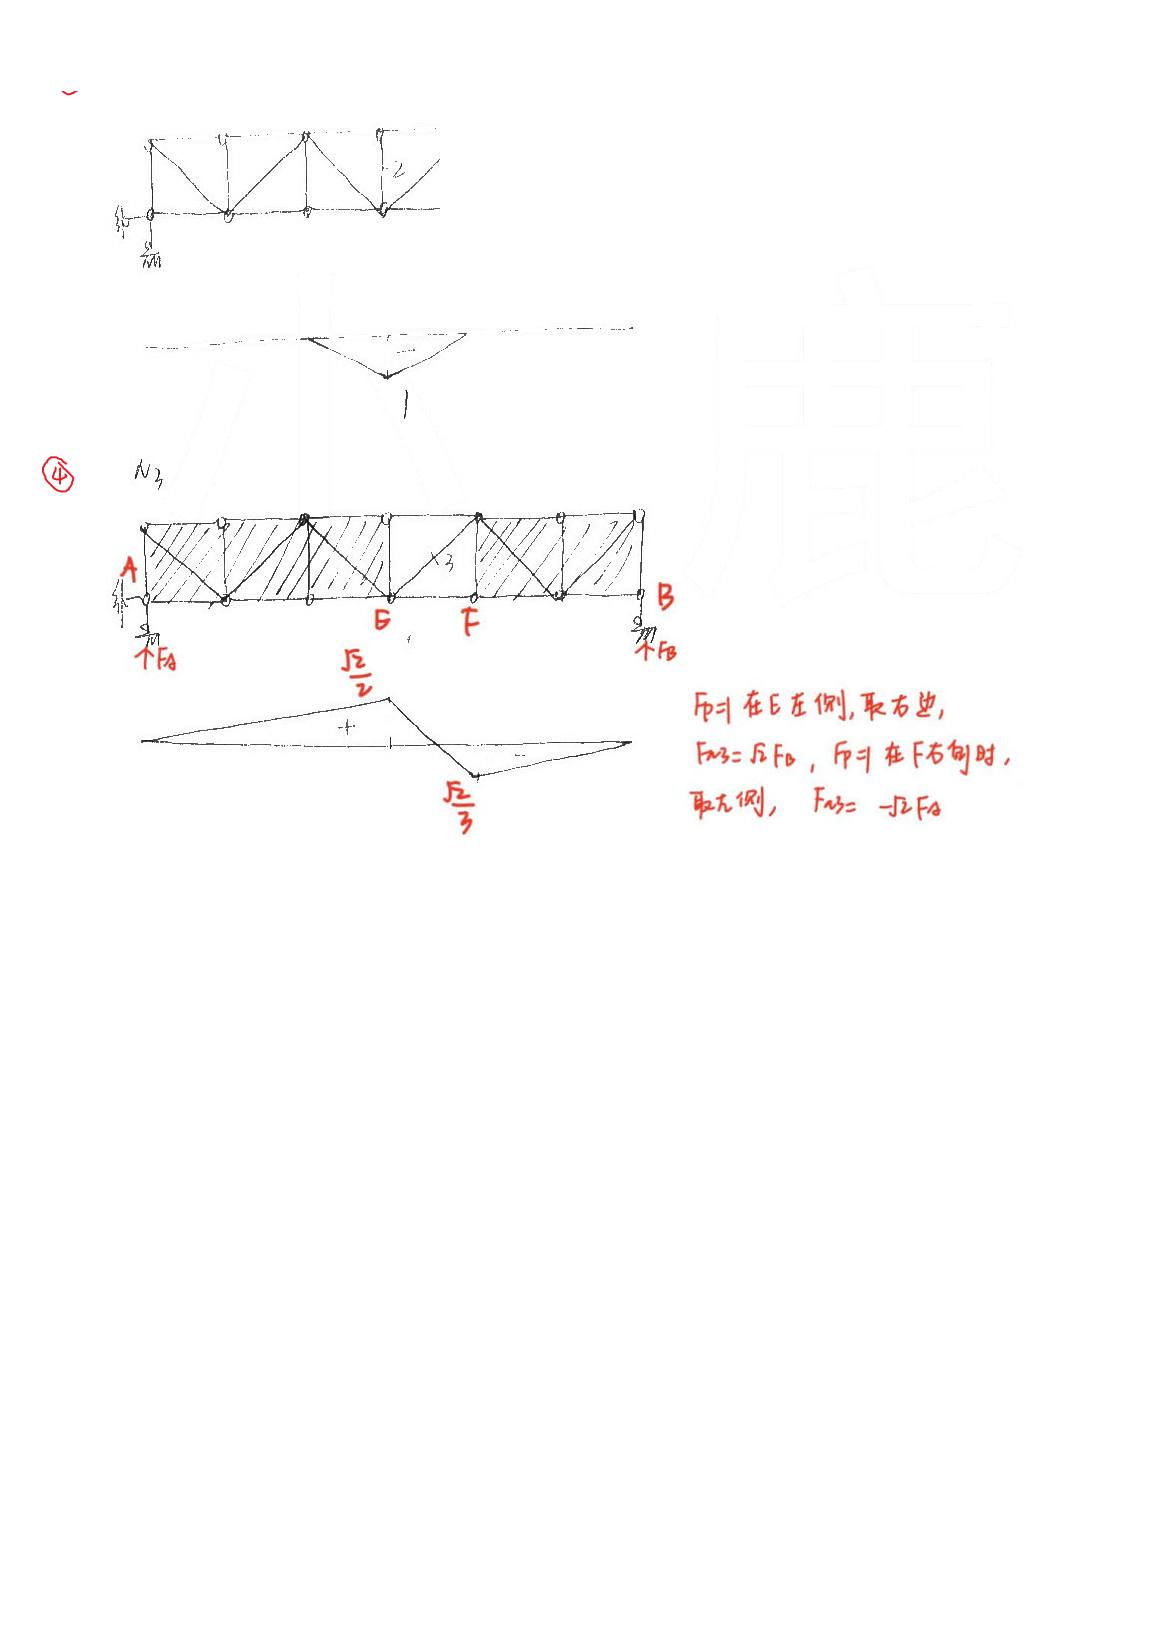
\includegraphics[width=0.92\textwidth]{figures/src11_p009.jpg}
\caption{结构力学基础与技巧班第8次作业及答案（静定结构影响线） 第 9 页清理图形页}
\end{figure}
\subsection*{第 10 页转写}
当单位力作用在下弦时

（1）

RA

F 杆轴力影响线

与作用在上弦相同，可直接画出单位力作用在下弦时

RA

F 影响线，如图（a）所示。

（2）1 杆轴力影响线

采用联合法，断开1 杆[见图（b）]。令断口两端发生单位相对位移，AC、DB 段影响线应分别保

持为直线，取A、C、D 和B 为关键点。当单位力作用在A 点和B 点时，力通过竖杆直接传递给大地了，

所以yA=yB=0。当单位力作用在C 点时，如图（c），求出支座反力，取 - 截面以右部分隔离体，根

据竖向力平衡可求出

1

2

6

N =

；当断开1 杆后，链杆IJ 和CD 相当于定向节点，因此AC 和BD 两段的

影响线应保持平行，根据AC 段影响线，可以求出单位力作用在D 点时

1

2 2

3

N =

。连接所有关键点竖

标，可得1 杆轴力影响线，如图（d）所示。

（3）2 杆轴力影响线（9 分）

当单位力作用在下弦时，2 杆始终为0 杆，影响线而（e ）所示
\begin{figure}[H]\centering
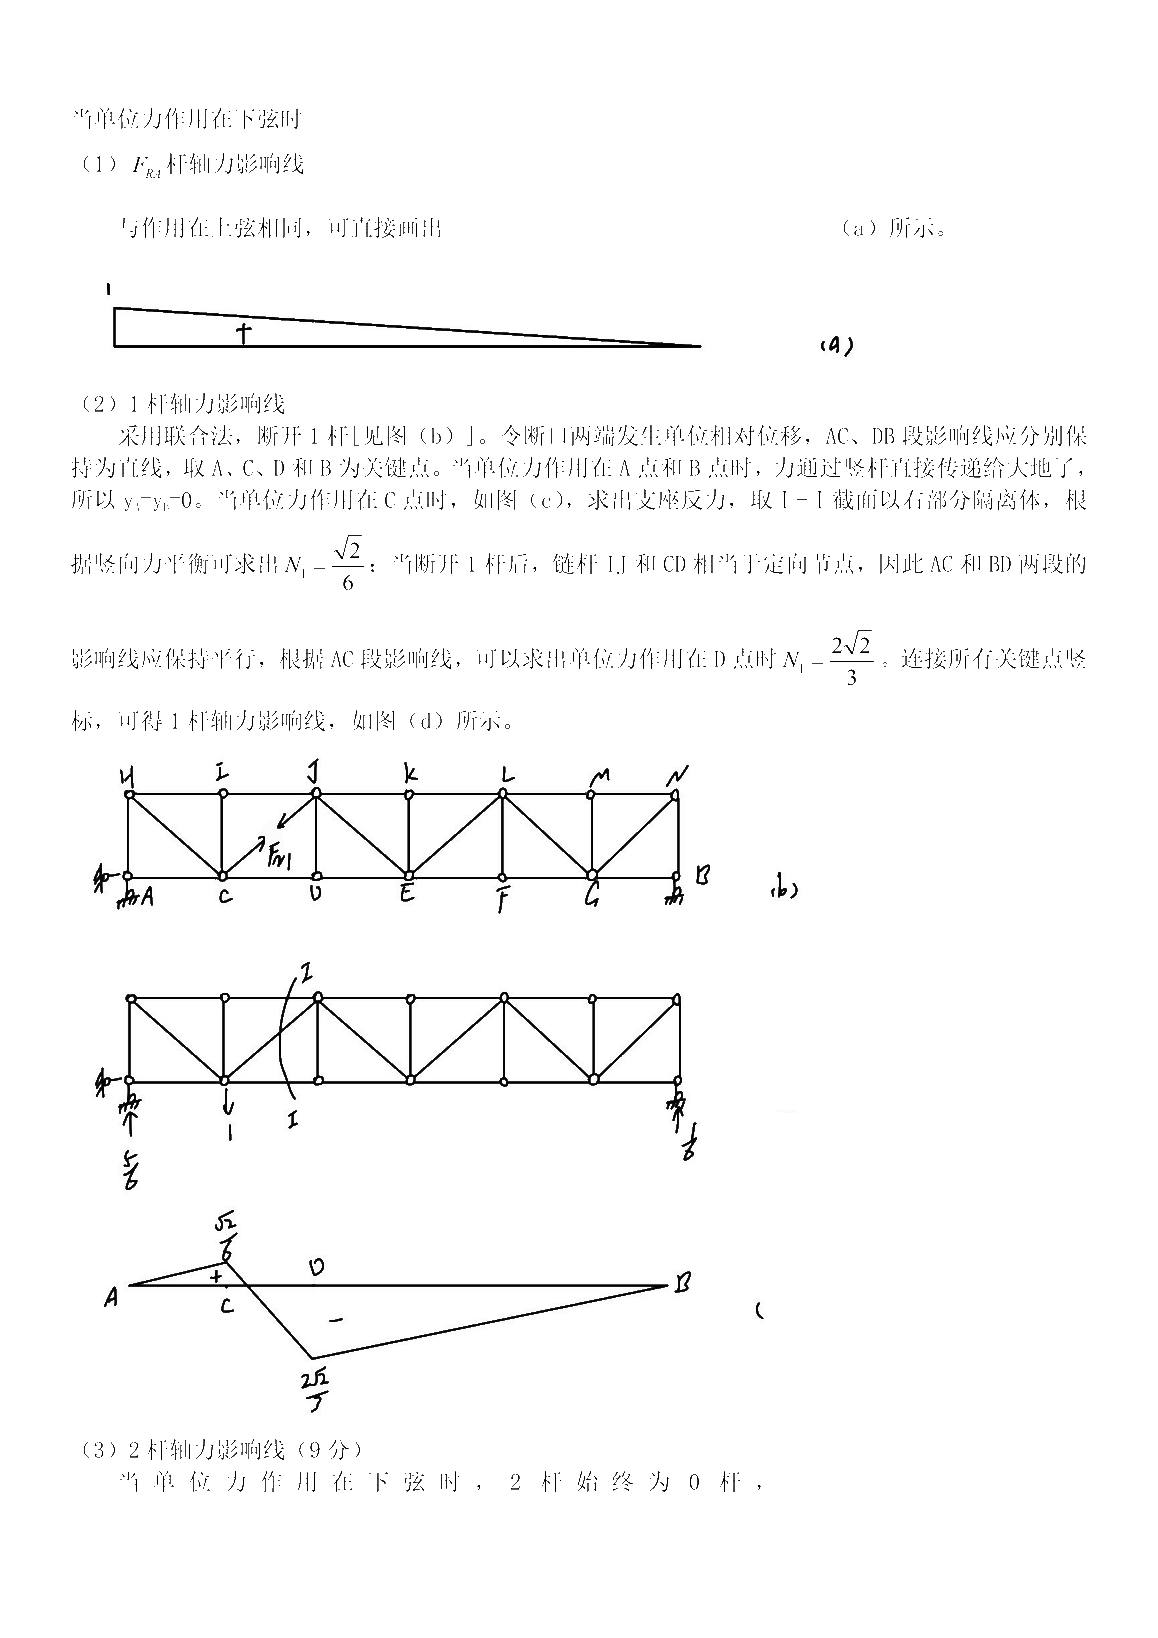
\includegraphics[width=0.92\textwidth]{figures/src11_p010.jpg}
\caption{结构力学基础与技巧班第8次作业及答案（静定结构影响线） 第 10 页清理图形页}
\end{figure}
\subsection*{第 11 页转写}
。

（4）3 杆轴力影响线

采用联合法，断开3 杆[见图（f）]。令断口两端发生单位相对位移，AE、BF 段影响线应分别保

持为直线，取A、E、B 和F 为关键点。当单位力作用在A 点和B 点时，力通过竖杆直接传递给大地了，

所以yA=yB=0。当单位力作用在E 点时，如图（g），求出支座反力，取 - 截面以右部分隔离体，根

据竖向力平衡可求出

3

2

2

N =

；当断开3 杆后，链杆KL 和EF 相当于定向节点，因此AE 和BF 两段的

影响线应保持平行，根据AE 段影响线，可以求出单位力作用在F 点时

3

2

3

N =

。连接所有关键点竖

标，可得3 杆轴力影响线，如图（h）所示。
\begin{figure}[H]\centering
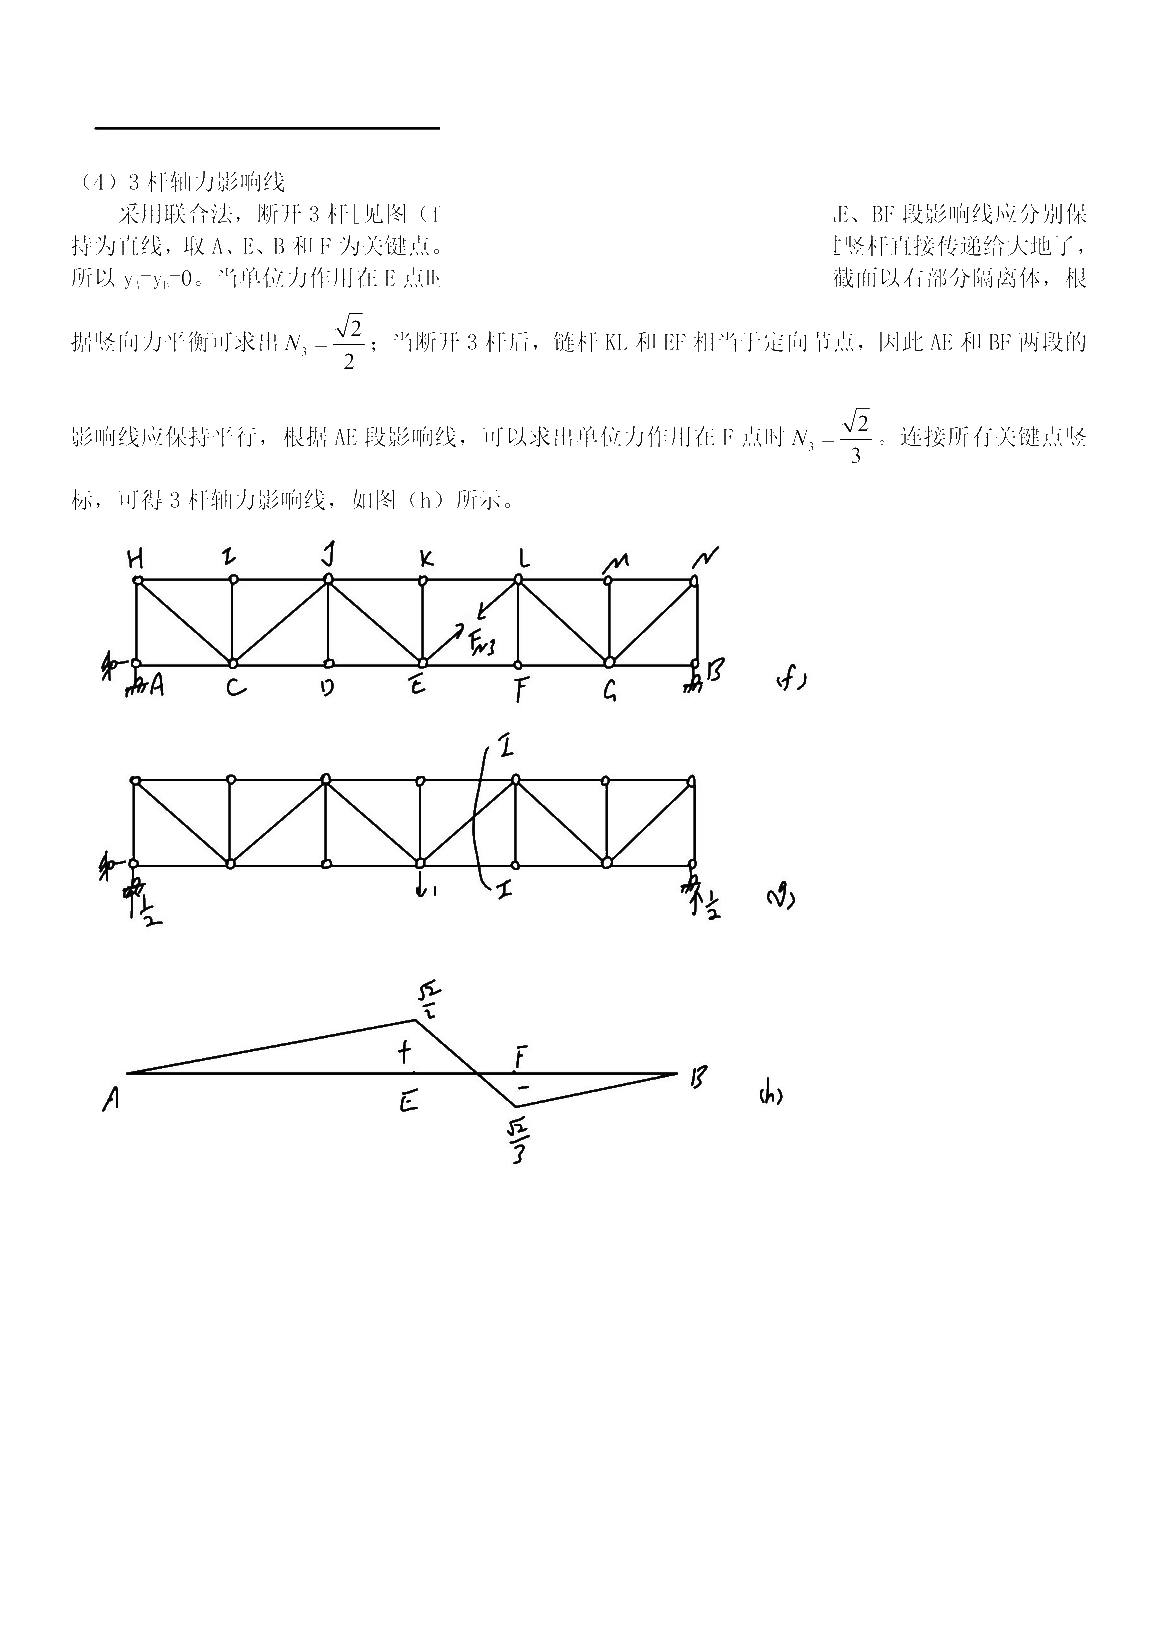
\includegraphics[width=0.92\textwidth]{figures/src11_p011.jpg}
\caption{结构力学基础与技巧班第8次作业及答案（静定结构影响线） 第 11 页清理图形页}
\end{figure}
\subsection*{第 12 页转写}
19
\begin{figure}[H]\centering
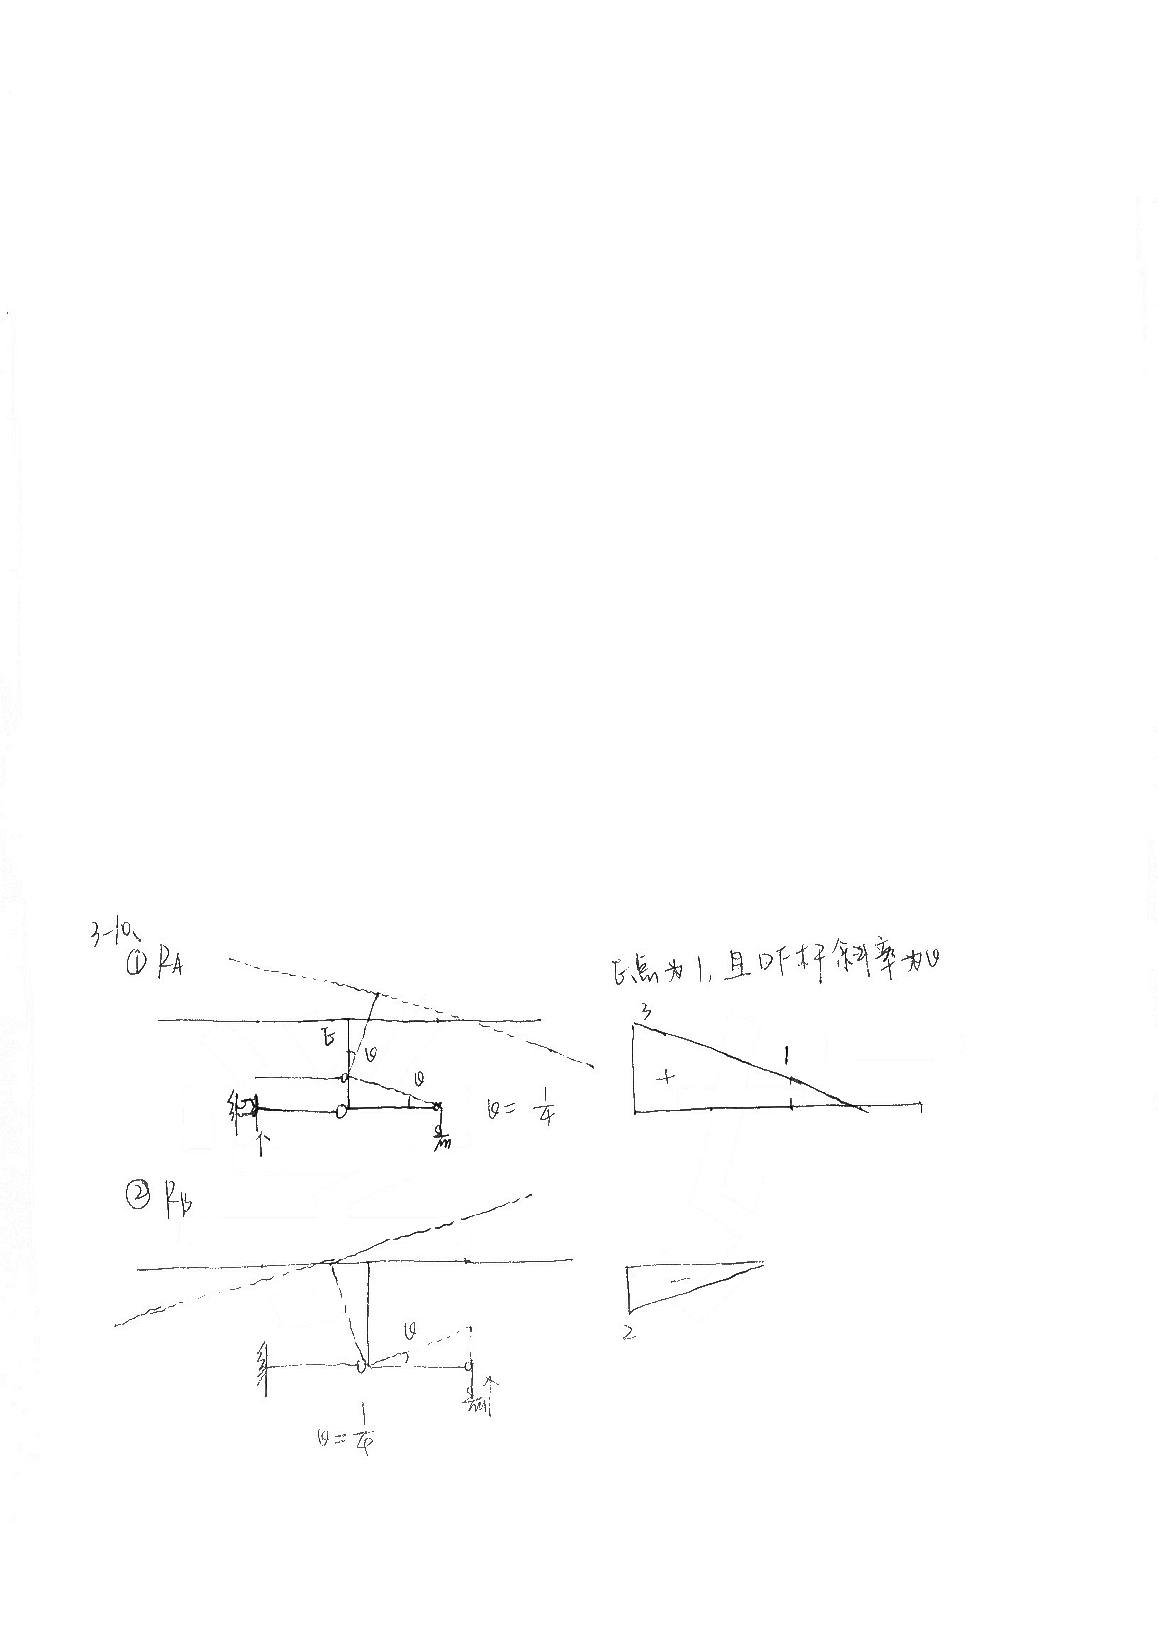
\includegraphics[width=0.92\textwidth]{figures/src11_p012.jpg}
\caption{结构力学基础与技巧班第8次作业及答案（静定结构影响线） 第 12 页清理图形页}
\end{figure}
\subsection*{第 13 页转写}
DF杆是个整体,位移后是身线

因此求西点即

M 2xey
\begin{figure}[H]\centering
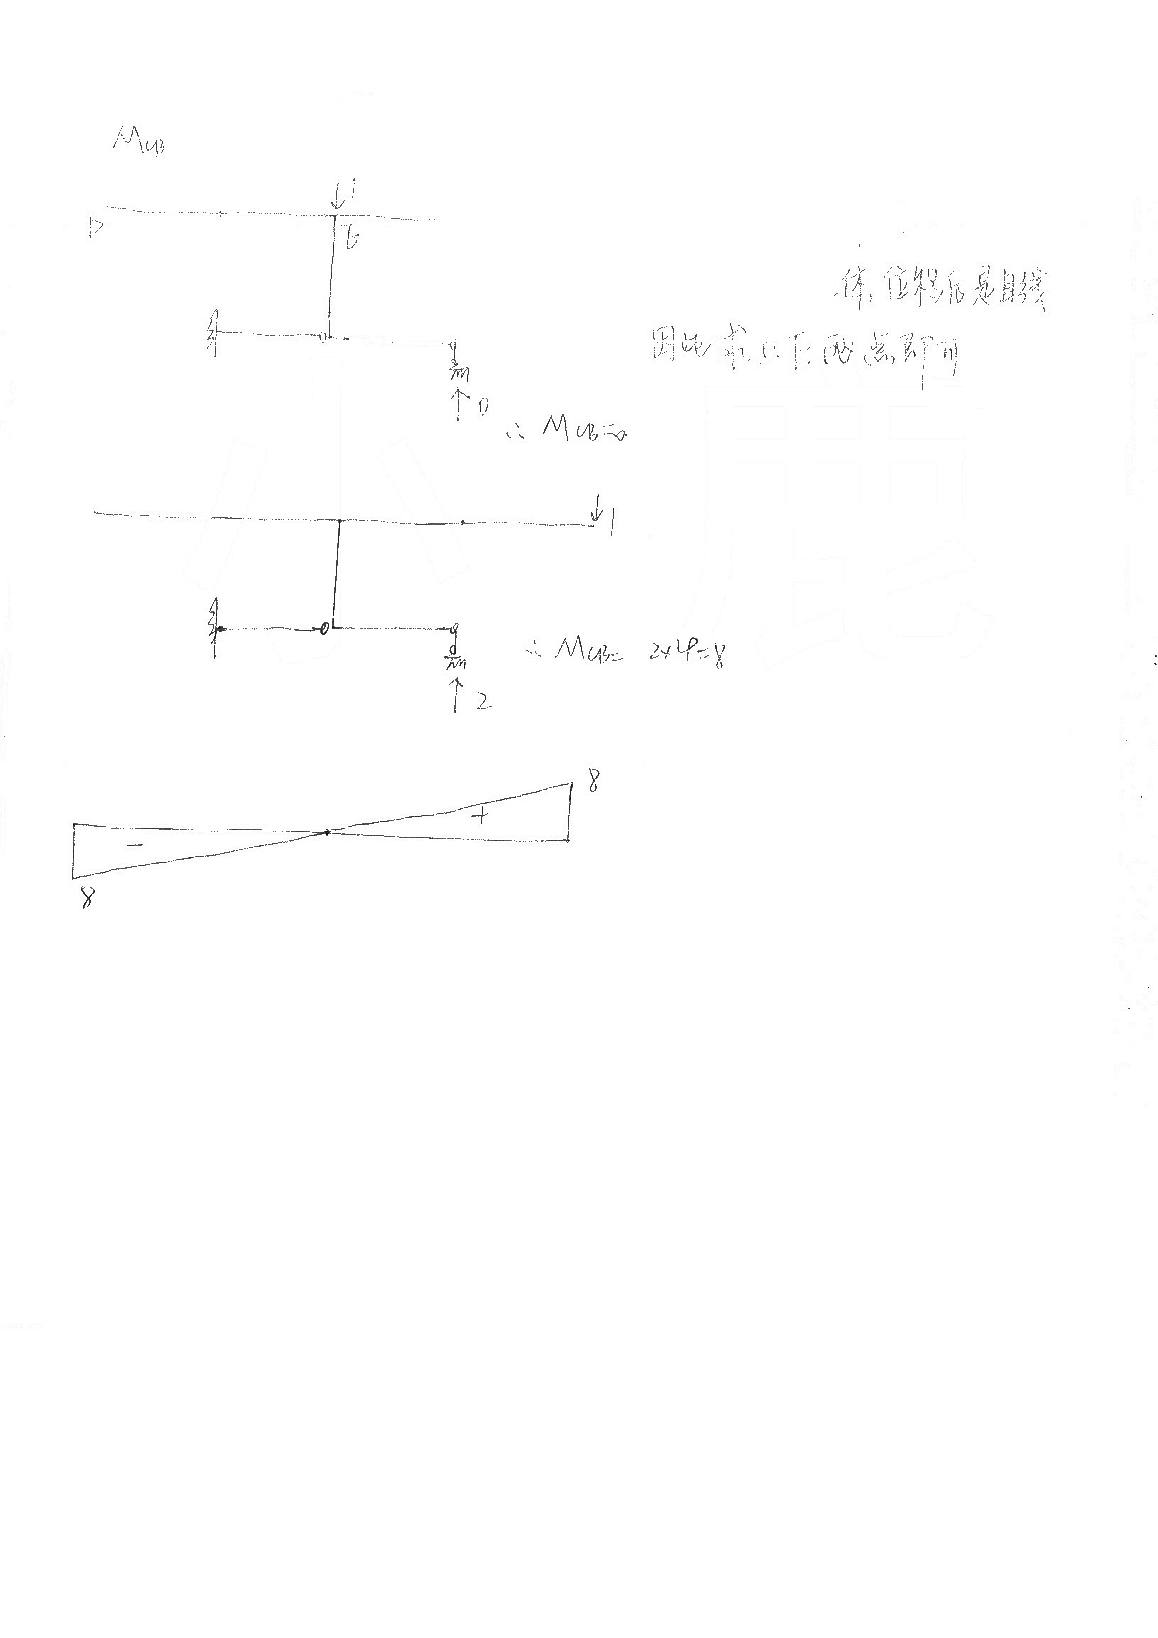
\includegraphics[width=0.92\textwidth]{figures/src11_p013.jpg}
\caption{结构力学基础与技巧班第8次作业及答案（静定结构影响线） 第 13 页清理图形页}
\end{figure}
\subsection*{第 14 页转写}
3-11、（1）

解：(1)

NDE

F

影响线

采用联合法，取B、C、D 为关键点，其中当单位力作用在B、C 点时DE 杆轴力为0.当单位力作用在D

点时如图（a）所示，根据结点D 竖向力平衡可得

5

4

NDE

F

=  

。综合以上计算，画出影响线如图（b）所示。

(2)

QBC

F

影响线

用机动法。去掉相应的约束，画出虚位移图[见图（c）]，令

QBC

F

对应的位移等于1，求出影响线的竖标

后可得到BC 杆B 端截面的剪力影响线如图（d）所示。

(3)

BC

M

影响线

用机动法。去掉相应的约束，画出虚位移图[见图（e）]，令

BC

M

对应的位移等于1，求出影响线的竖标

后可得到BC 杆B 端截面的弯矩影响线如图（f）所示。

（2）图示荷载作用下，可分别求得DE 杆轴力和

BC

M

为

1

5

15

3

4

2

4

2

NDE

F

KN

=  

\textbackslash{}times \textbackslash{}times

\textbackslash{}times

=  

，

1 3 3 4

18

2

BC

M

KN m

=  

\textbackslash{}times \textbackslash{}times \textbackslash{}times

=  


\begin{figure}[H]\centering
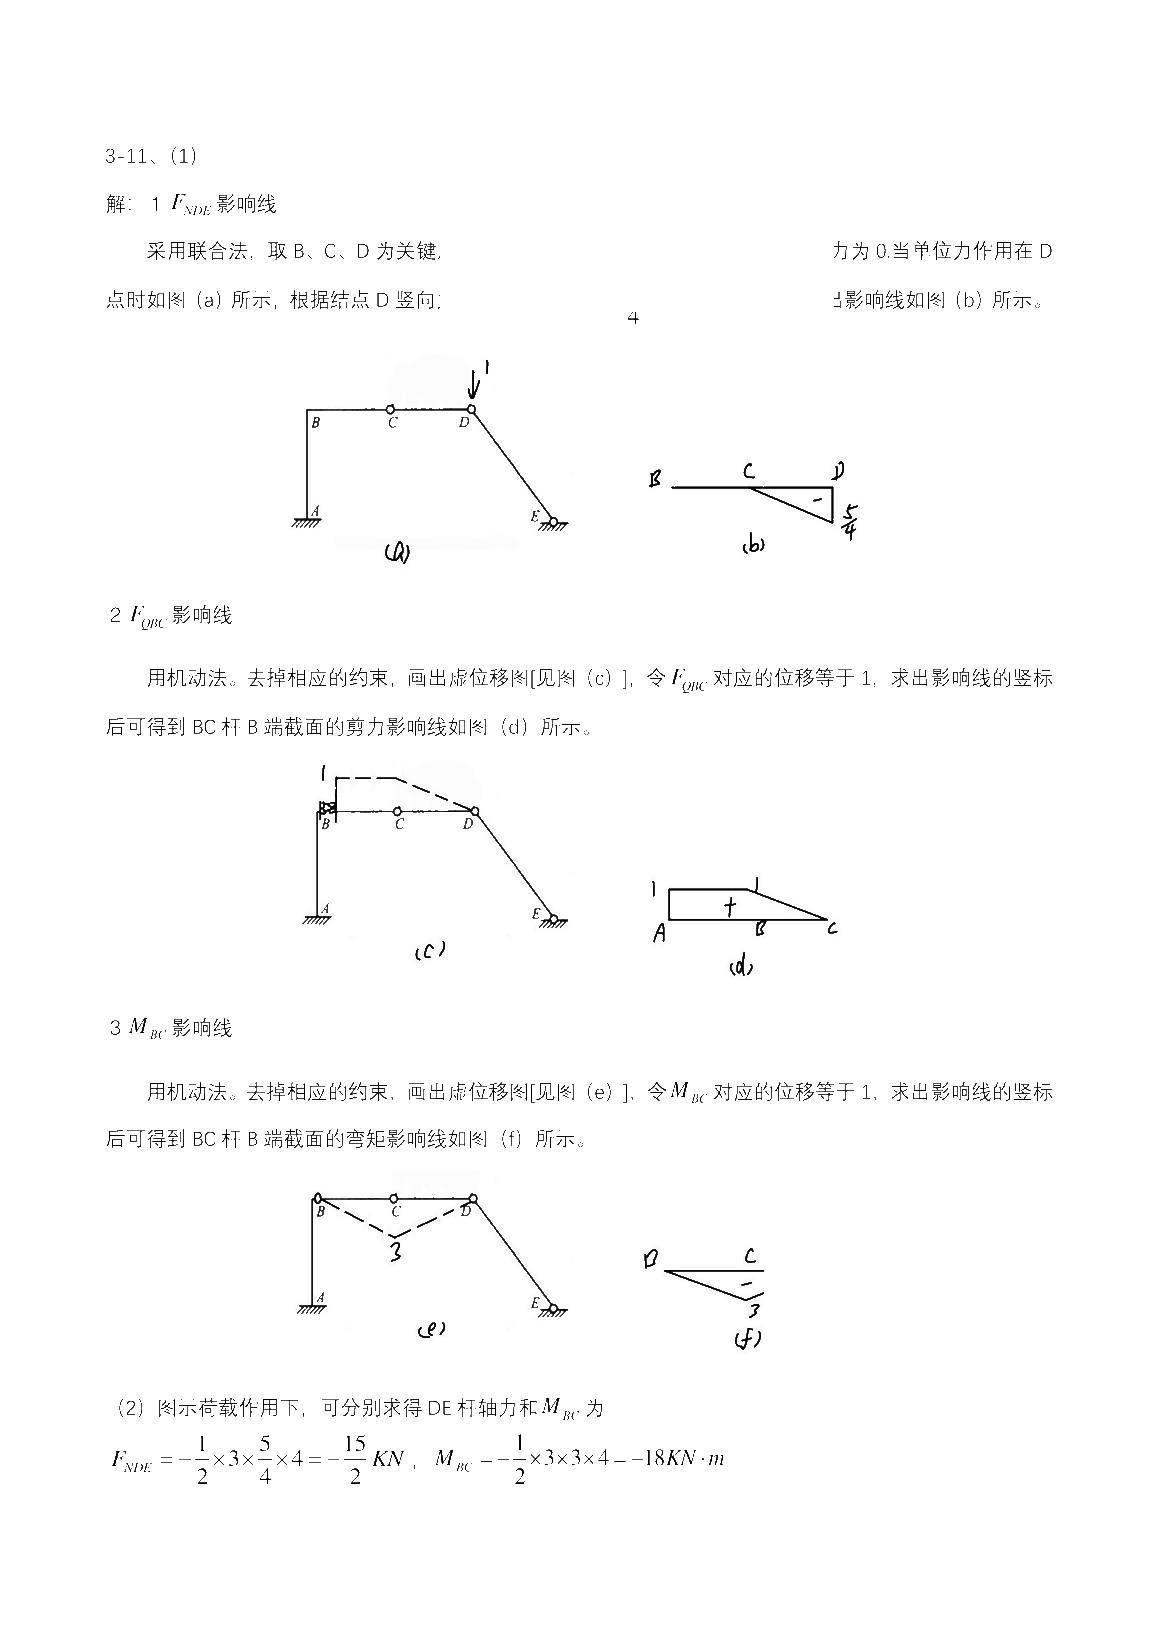
\includegraphics[width=0.92\textwidth]{figures/src11_p014.jpg}
\caption{结构力学基础与技巧班第8次作业及答案（静定结构影响线） 第 14 页清理图形页}
\end{figure}
\subsection*{第 15 页转写}
312、

作用时，NNAB
\begin{figure}[H]\centering
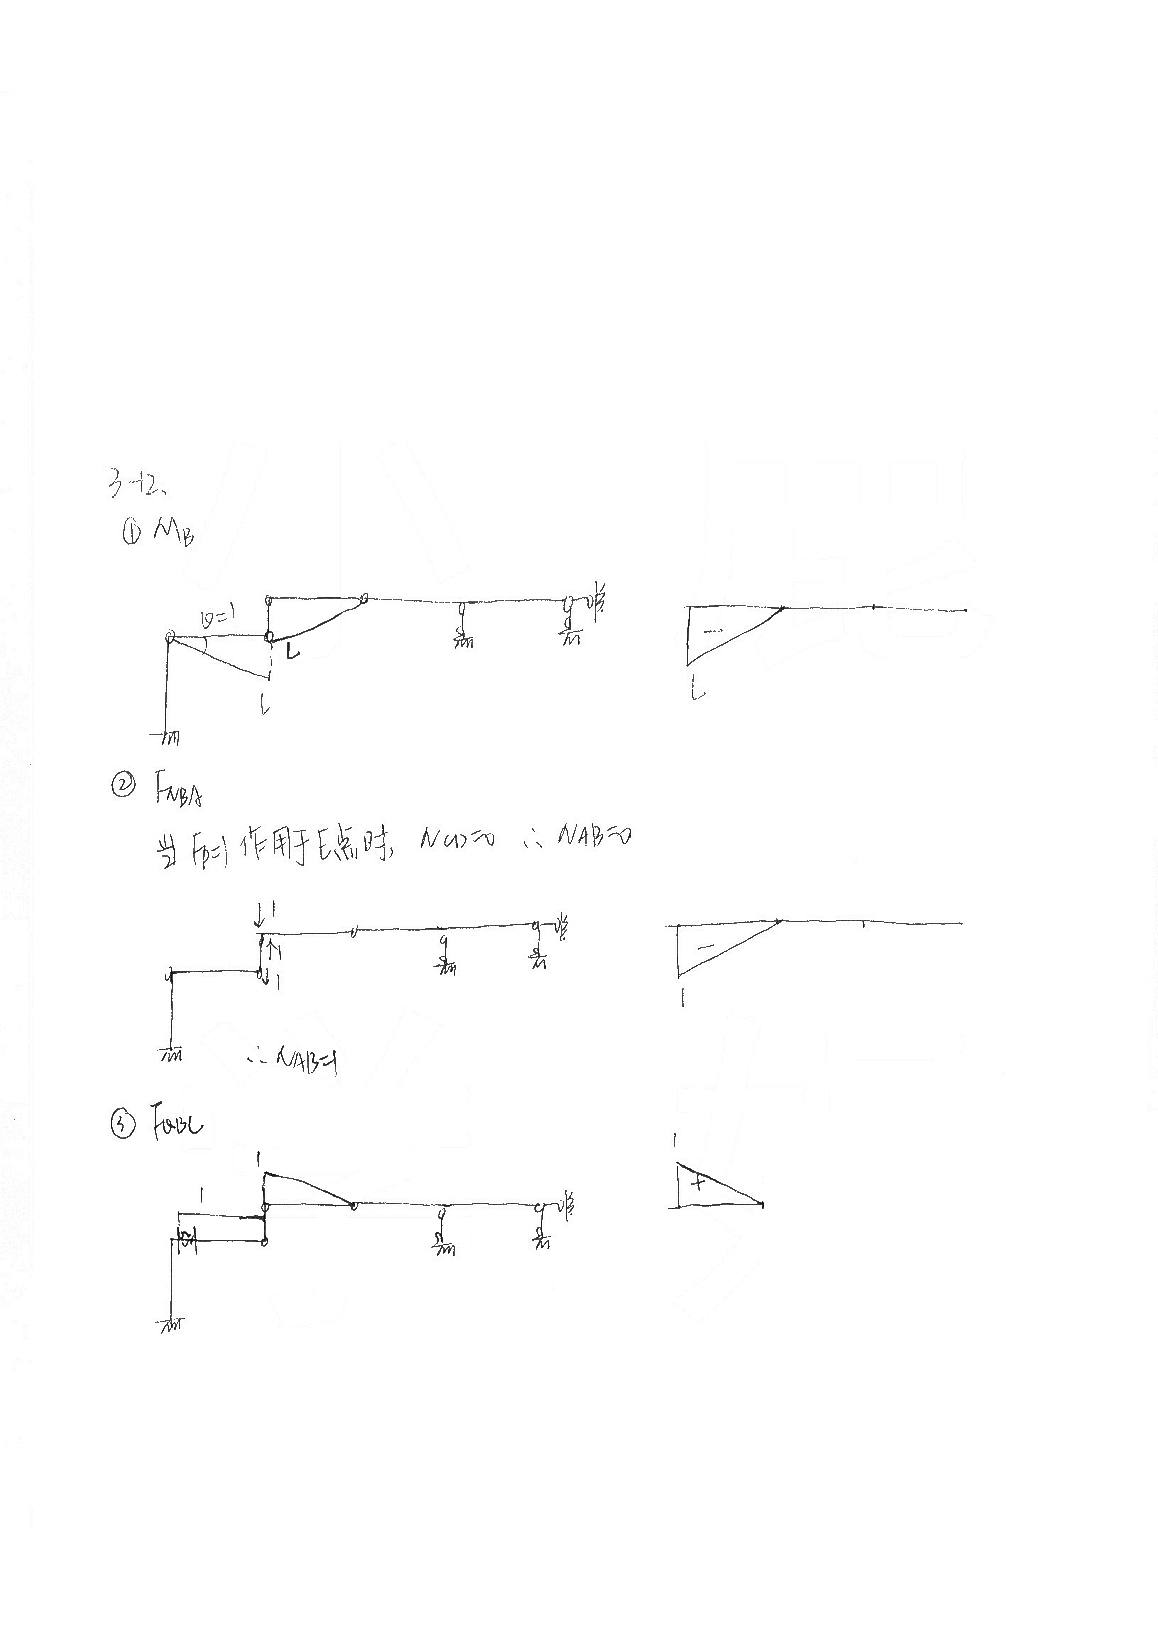
\includegraphics[width=0.92\textwidth]{figures/src11_p015.jpg}
\caption{结构力学基础与技巧班第8次作业及答案（静定结构影响线） 第 15 页清理图形页}
\end{figure}
\subsection*{第 16 页转写}
3-3、作处，=

作，M

布作用于处

M作CID时，Fk0。

Mc-0

NEF$\times$3=X* NBF-

MB向线

以恒为男，因地彩同线为0

M影线
\begin{figure}[H]\centering
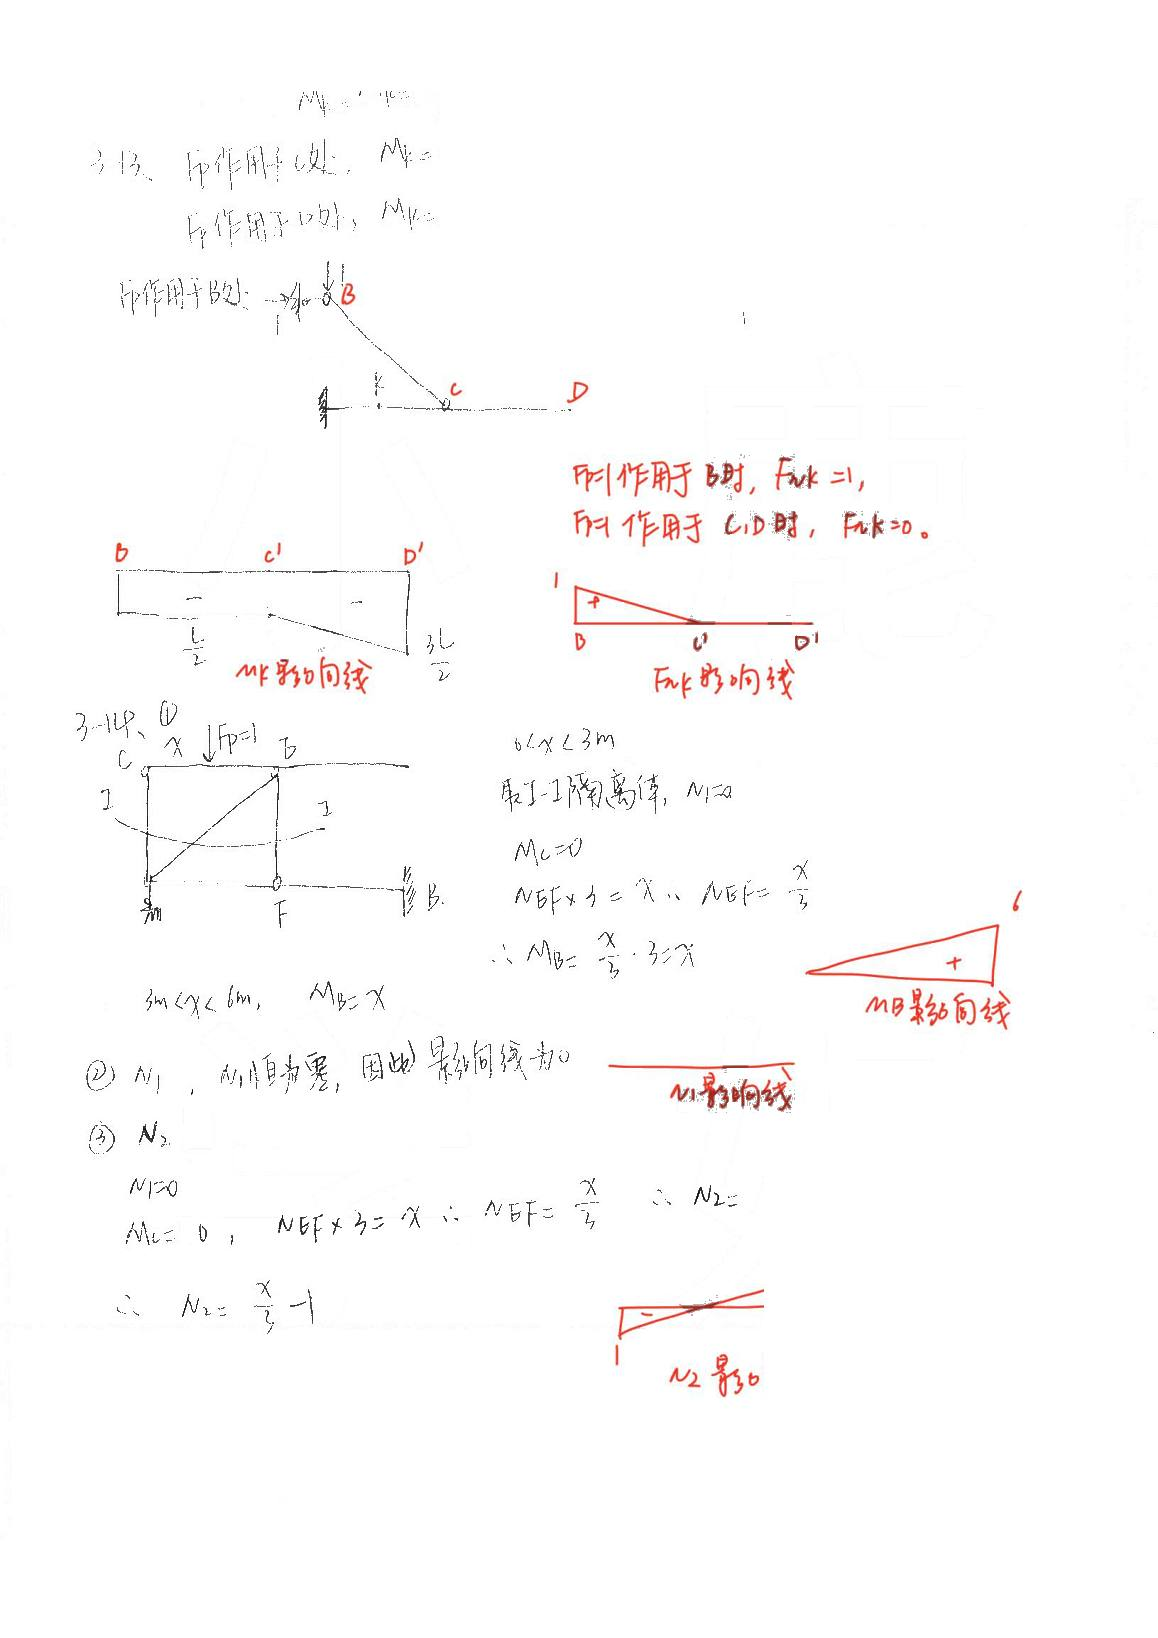
\includegraphics[width=0.92\textwidth]{figures/src11_p016.jpg}
\caption{结构力学基础与技巧班第8次作业及答案（静定结构影响线） 第 16 页清理图形页}
\end{figure}
\subsection*{第 17 页转写}
315

27X70

MAEO

Fx+\$

MAZO

(2) Tms

3-b-

(0)

4m

30
\begin{figure}[H]\centering
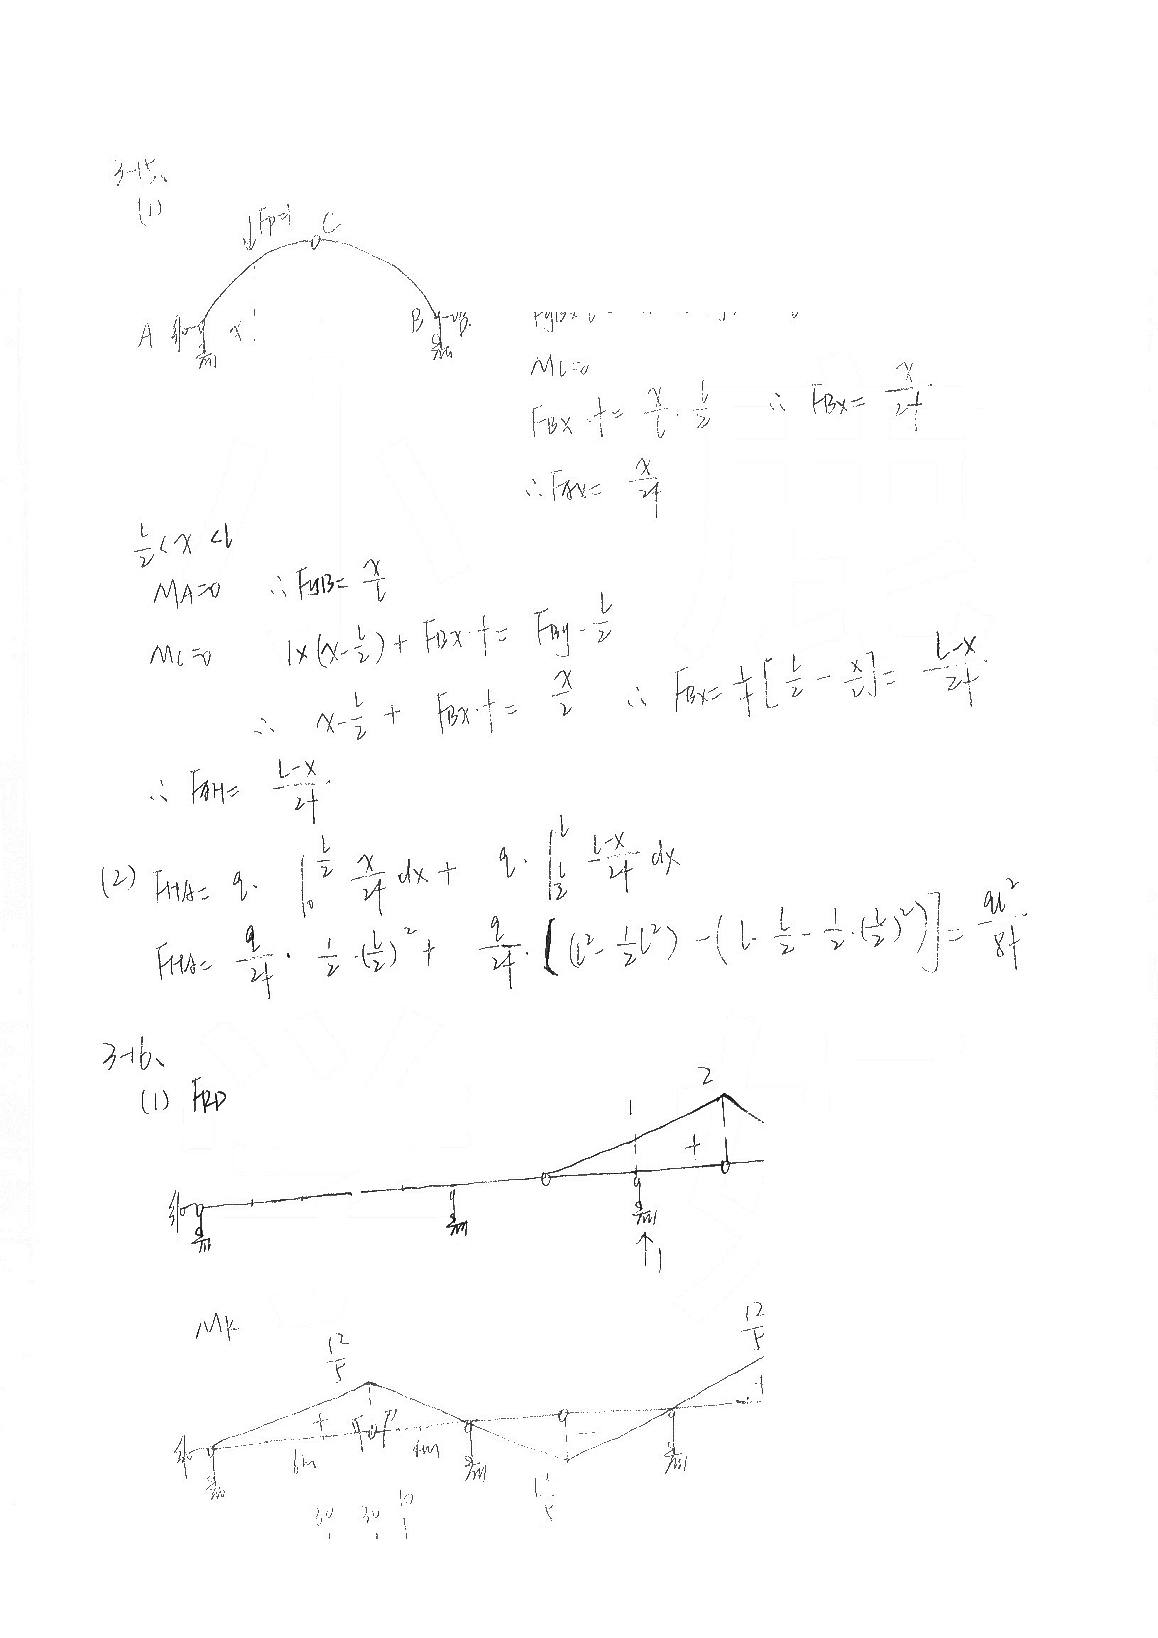
\includegraphics[width=0.92\textwidth]{figures/src11_p017.jpg}
\caption{结构力学基础与技巧班第8次作业及答案（静定结构影响线） 第 17 页清理图形页}
\end{figure}
\subsection*{第 18 页转写}
（30x+30x+1072+718=m
\begin{figure}[H]\centering
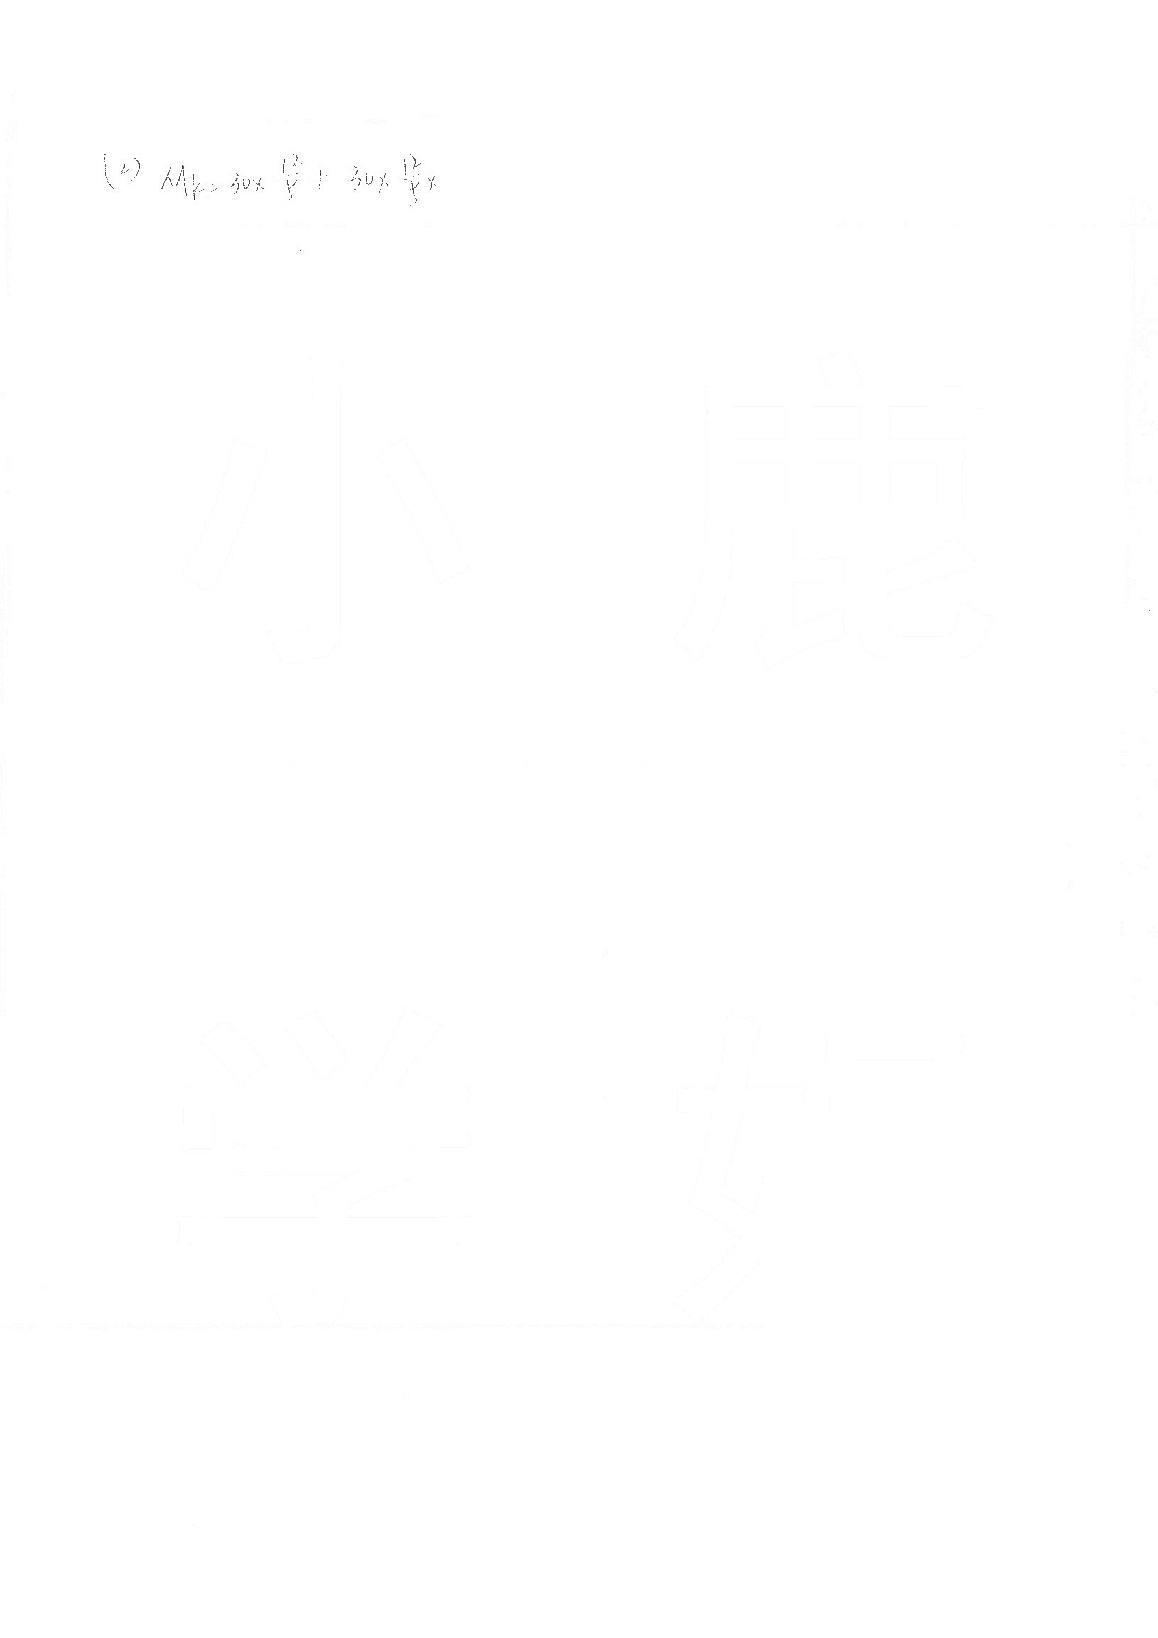
\includegraphics[width=0.92\textwidth]{figures/src11_p018.jpg}
\caption{结构力学基础与技巧班第8次作业及答案（静定结构影响线） 第 18 页清理图形页}
\end{figure}
